\documentclass[journal,onecolumn]{IEEEtran}
\usepackage{amsmath,amssymb,booktabs,array,longtable,graphicx,url}
\usepackage[hidelinks]{hyperref}
\usepackage[section]{placeins}
\title{Research Compendium: Service-Relative Physical--Virtual Fidelity in Sensor-Lightweight Digital Twins}
\author{Shreyas Udaya}

\begin{document}
\maketitle

\begin{abstract}
This compendium documents experiments on physical--virtual fidelity in sensor-lightweight digital twins. The work begins with a mobile-robot twin driven by wheel and inertial measurements, separates short-horizon trajectory agreement from accumulated global synchronization, and studies how benign operating condition changes the fidelity profile. It then defines service-relative contracts over required quantities, horizons, physical tolerances, freshness limits, and observability. Experiments use ten i2Nav robot sequences with three frozen-model seeds, AprilTag-referenced UGV01 recordings, five TerraSentia agricultural-robot sequences, twenty UGV01 live telemetry traces, and thermal and process datasets. Completed evidence shows that low finite-horizon relative error can coexist with large global divergence; persistent yaw mismatch is associated with accumulated heading and position error; fidelity distributions vary with turning, acceleration, curvature, wheel--IMU disagreement, and elapsed time; and sampled delivery can change whether an already-computed twin state satisfies a service without changing the underlying model. Negative findings include weak transfer of a frozen i2Nav model to TerraSentia, poor cross-run transfer of a same-run UGV01 calibration, transport-rate collapse in the live UGV01 prototype, and unavailable causal timing provenance in MAGNET. Doubly nested leave-one-sequence-out training, causal-derivative retraining, and Linux network emulation are documented separately as incomplete experiments and are not included in completed-result claims.
\end{abstract}

\begin{IEEEkeywords}
digital twin, physical--virtual fidelity, service contract, trajectory evaluation, age of information, mobile robot, condition dependence, observability
\end{IEEEkeywords}

\section{Introduction}
A digital twin is a computational representation whose value depends on whether its state is sufficiently close to a physical asset for a specified use. A single scalar accuracy number is inadequate for this purpose. A robot may preserve local motion over one or five seconds while accumulating a large global pose offset. A state may also be physically accurate at its source timestamp yet arrive too late for a service that requires recent information. Conversely, a service may fail even under ideal delivery because the twin model itself has diverged.

This project studies these distinctions in a sensor-lightweight setting. The primary robot twin uses wheel and inertial information rather than camera, LiDAR, radar, or GNSS as learned-model inputs. Its outputs are compared with physical references using componentwise position, heading, velocity, yaw-rate, finite-horizon relative pose, and accumulated-residual quantities. The same discrepancies are then evaluated against service-specific quantity, horizon, tolerance, freshness, and observability requirements.

The experimental record spans model development, frozen cross-sequence evaluation, mechanism analysis, condition-dependent characterization, physical UGV01 instantiation, external-platform transfer, sampled-delivery replay, live telemetry, and cross-domain fidelity studies. Physical sequences are the primary statistical units. Random seeds quantify model variability for the same sequence; timestamps, replay cells, services, and delivery phases do not create additional independent physical experiments.

\subsection{Contributions}
The completed work provides the following contributions:
\begin{enumerate}
\item A componentwise fidelity framework that keeps local relative-pose error, global physical--virtual divergence, rate disagreement, and accumulated residuals in their physical units rather than collapsing them into one weighted score.
\item An empirical demonstration that local and global fidelity can rank the same physical sequences differently, together with a measurable yaw-divergence pathway from persistent rate mismatch to heading and position divergence.
\item A condition-dependent benign fidelity characterization based on speed, acceleration, turning, curvature, wheel--IMU disagreement, and elapsed time, including leave-one-sequence-out stability analysis.
\item A service contract that joins physical discrepancy, freshness, and observability and distinguishes delivery-remediable cases from persistent model discrepancy.
\item A multi-source experimental record covering i2Nav, UGV01, TerraSentia, MAGNET, FreeTwinEV, and TU Wien SNG, with independent-reference, fused-reference, replay, simulation, and negative results explicitly separated.
\end{enumerate}

\section{Related Work}
Digital-twin literature has emphasized definitions, architectures, synchronization, credibility, and application-specific value. Jones \emph{et al.} organize the conceptual properties of digital twins, while Shao \emph{et al.} emphasize credibility as a property that must be justified for an intended use \cite{jones2020,shao2023}. The present work operationalizes this idea through componentwise, service-relative physical--virtual evidence.

Trace-alignment fidelity compares physical and virtual event traces and provides a general framework for measuring correspondence \cite{munoz2024}. Mobile-robot studies also compare simulated and physical navigation behavior \cite{bergs2025}. The current framework differs by retaining synchronized physical units, multiple trajectory horizons, observability, and sampled-delivery freshness in one contract representation.

Age of Information, Age of Incorrect Information, and query-oriented freshness formalize the value of timely updates \cite{maatouk2023,chiariotti2022}. Digital-twin synchronization work studies when updates should occur under communication or synchronization cost \cite{tanmatta2024,li2025sync}. The present experiments do not derive an optimal synchronization policy. They test whether delivered states satisfy explicit physical and freshness requirements and separate failures that can be changed by delivery from those that remain under ideal available delivery.

Wheel--inertial odometry and learned residual correction motivate the sensor-lightweight twin \cite{brossard2019,jiang2025,zhou2025ynet}. The learned model is not compared as a replacement for camera- or LiDAR-based localization. Instead, it is used to expose how model errors evolve under benign operation and how those errors interact with service requirements. i2Nav provides the main ten-sequence robot corpus \cite{tang2025}; TerraSentia provides a distinct agricultural skid-steer platform \cite{cuaran2024}; and AprilTag supplies an independent planar reference for UGV01 experiments \cite{olson2011}.

Thermal and process datasets test whether the component--horizon--tolerance representation remains meaningful outside robot pose. MAGNET is used for target-aligned thermal forecast fidelity, with forecast target offsets kept distinct from unverified forecast issue or arrival time \cite{wilsdon2023magnet}.

\section{Framework and Methodology}
\subsection{Twin state and physical reference}
Let the physical reference and twin state be
\begin{equation}
\mathbf{x}_{P}(t)=[x_P,y_P,\theta_P,v_P,\omega_P]^\top,\qquad
\mathbf{x}_{T}(t)=[x_T,y_T,\theta_T,v_T,\omega_T]^\top .
\end{equation}
The evaluated source of $\mathbf{x}_{P}$ depends on the experiment: i2Nav ground truth, AprilTag pose, TerraSentia RTK position, or another documented physical/reference stream. A fused estimate is labeled as a diagnostic reference rather than independent ground truth.

\subsection{Componentwise fidelity}
Global position and heading disagreement are
\begin{align}
D_p(t)&=\left\|\mathbf{p}_T(t)-\mathbf{p}_P(t)\right\|_2,\\
D_\theta(t)&=\left|\operatorname{wrap}\!\left(\theta_T(t)-\theta_P(t)\right)\right|.
\end{align}
Rate disagreement uses $D_v(t)=|v_T-v_P|$ and $D_\omega(t)=|\omega_T-\omega_P|$. Finite-horizon relative pose error at horizon $h$ compares physical and virtual motion increments over $[t,t+h]$. Reported horizons are 1, 5, and 10 s where trajectory duration and reference continuity support them. ATE, heading MAE, percentile and maximum divergence, persistent signed yaw residual, and accumulated yaw residual $I_\omega$ provide complementary summaries. Meters, degrees, meters per second, and radians per second remain separate dimensions.

\subsection{Condition-dependent benign characterization}
For benign hypothesis $H_0$ and operating context $c$,
\begin{equation}
D(t)\mid H_0,c \sim P_{\mathrm{benign}}(D\mid c).
\end{equation}
The descriptive componentwise percentile set is
\begin{equation}
\mathcal{E}_{\mathrm{benign}}^{(q)}(c)=
\left\{D:\ D_j\le Q_q[D_j\mid H_0,c]\ \text{for every supported component }j\right\}.
\end{equation}
The $q=0.95$ summaries characterize the observed benign data; exceeding them does not by itself imply an attack, anomaly, failure, or loss of trust.

\subsection{Service-relative contract}
A service $s$ is specified by required components $Q_s$, horizon $h_s$, component tolerances $\boldsymbol{\delta}_s$, freshness limit $\Delta_s$, satisfaction requirement $\rho_s$, and observability rule. For an observable delivered state at evaluation time $t_k$,
\begin{equation}
V_{s,k}=
\mathbb{I}\!\left[
D_j(t_k;h_s)\le\delta_{s,j}\ \forall j\in Q_s
\ \land\ 
\operatorname{AoI}_k\le\Delta_s
\right].
\end{equation}
If the required reference quantity is unavailable, $V_{s,k}=\varnothing$. The aggregate service state is computed only over eligible observable samples. Thus pass, fail, and unobservable are distinct outcomes.

\subsection{Delivery replay and remediability}
Saved source states are released according to a specified source rate, delay, jitter, loss process, and receiver rule. A case that fails under degraded delivery but passes under ideal available delivery is delivery-remediable. A case that still fails under ideal delivery has persistent model discrepancy. A case already passing under degraded delivery is already qualified. Newer delivery can change the discrepancy of a held state at evaluation time, but it does not alter the frozen model trajectory.

\subsection{Statistical hierarchy}
The hierarchy is
\[
\text{timestamps}\subset\text{seed run}\subset\text{physical sequence}\subset\text{dataset}.
\]
Metrics are computed within a seed run, seeds are aggregated within a physical sequence, and physical sequences are used for dataset-level inference. Bootstrap and sign-flip procedures resample or flip at the physical-sequence level.

\section{Detailed Experimental Methodology}
\subsection{End-to-end study organization}
The study is organized as a sequence of frozen transformations:
\begin{enumerate}
\item construct a time-aligned physical/reference stream and a sensor-only virtual-state input stream;
\item train or instantiate a twin without using the evaluated sequence as an input source;
\item save the complete virtual trajectory and its rate outputs;
\item evaluate local, global, rate-domain, and accumulated-residual fidelity;
\item stratify the saved discrepancies by benign operating context;
\item replay sampled delivery without changing the saved source trajectory;
\item evaluate service contracts and aggregate seeds within physical sequence; and
\item repeat the evaluator on physical UGV01, TerraSentia, and non-robot datasets wherever the required reference quantities exist.
\end{enumerate}
Training, physical-reference evaluation, delivery replay, and cross-domain transfer are separate stages. Ground truth may supervise training on training sequences and evaluate held-out sequences, but it is not supplied as a runtime feature to the learned i2Nav twin.

\subsection{Data sources and reference roles}
Table~\ref{tab:data-method} records the role of each principal dataset. An independent physical reference supports direct fidelity claims. A fused estimate is used only for secondary mechanism diagnostics. Saved-state replay tests delivery effects over an already-generated trajectory and does not create new physical motion.

\begin{longtable}{p{.18\linewidth}p{.22\linewidth}p{.24\linewidth}p{.27\linewidth}}
\caption{Data sources and methodological roles.}\label{tab:data-method}\\
\toprule
Source & Twin/runtime inputs & Evaluated reference & Use \\
\midrule\endfirsthead
\toprule
Source & Twin/runtime inputs & Evaluated reference & Use \\
\midrule\endhead
i2Nav & Odometer speed and IMU yaw dynamics & Dataset navigation ground truth & Model development, frozen LOSO fidelity, conditions, envelopes, services, and official benchmark. \\
UGV01 AprilTag & Encoders, IMU, commands, and timing & ChArUco-calibrated fixed AprilTags and rover tag & Asset-specific calibration, physical trajectory fidelity, and frozen holdouts. \\
TerraSentia & Four motor-speed fields and robot IMU & RTK position; fused EKF only for secondary yaw diagnostics & Deterministic adapter and external-platform transfer. \\
UGV01 live & Dashboard telemetry, GPS, policy and transport logs & GPS for operational observability; matched video retained separately & Live contract plumbing, delivered-rate audit, and trace replay. \\
MAGNET & Saved thermal forecast fields & Measured heat-pipe temperatures & Target-aligned thermal fidelity by component and within-window target offset. \\
FreeTwinEV and TU Wien SNG & Saved simulated or soft-sensor quantities & Paired experimental/process quantities & Structural transfer of the component--horizon--tolerance representation. \\
\bottomrule
\end{longtable}

\subsection{i2Nav canonical preparation}
Each i2Nav sequence is converted to a common 10-Hz clock. Odometer speed and IMU yaw rate form the nominal planar propagation inputs. The six learned-model features are odometer speed, IMU yaw rate, odometer acceleration, IMU yaw acceleration, absolute yaw rate, and absolute odometer acceleration. Position, heading, GNSS coordinates, innovations, NIS, covariance, and reported GNSS uncertainty are excluded from learned inference.

The canonical state uses a local ENU/FLU-style planar representation internally. Heading is unwrapped for interpolation and wrapped only for angular differences. Evaluation trajectories retain their common physical frame; no post-hoc spatial alignment is applied in the internal fidelity analysis. The official i2Nav benchmark uses its separately verified NED/TUM conversion and SE(3) alignment protocol.

Acceleration and yaw acceleration in the completed frozen bank were constructed with centered numerical gradients. This can require the next 10-Hz sample, corresponding to a 100-ms feature-availability boundary. The completed lookahead-as-delay study accounts for that boundary in delivery replay. The separate causal-derivative experiment recomputes features with backward differences and retrains the model; it is incomplete.

\subsection{Frozen V2 model and propagation}
The frozen model separates fast motion correction from persistent yaw correction. The fast branch consumes a 20-sample, 2-s window of the six canonical features. It uses a two-layer GRU with 64 hidden units, 0.1 inter-layer dropout, and layer normalization. Two bounded linear heads predict
\begin{align}
\Delta v_k&=0.15\tanh(z_{v,k}),\\
\Delta\omega_{\mathrm{fast},k}&=0.020\tanh(z_{\omega,k}).
\end{align}
A separate slow branch uses 16 causal statistics over the previous 30 s: mean, standard deviation, RMS, and mean magnitude of IMU yaw and wheel-yaw proxy; mean, standard deviation, and RMS wheel--IMU yaw disagreement; mean and standard deviation of normalized disagreement; and mean, standard deviation, and mean magnitude of forward speed. A two-layer 32-unit tanh MLP predicts one bounded additive yaw state
\begin{equation}
b_{\mathrm{slow},k}=0.005\tanh(z_{\mathrm{slow},k}),\qquad
\Delta\omega_k=\Delta\omega_{\mathrm{fast},k}+b_{\mathrm{slow},k}.
\end{equation}

The corrected motion input and planar propagation are
\begin{align}
v_{T,k}&=v_{\mathrm{odo},k}+\Delta v_k,\\
\omega_{T,k}&=\omega_{\mathrm{imu},k}+\Delta\omega_k,\\
\theta_{T,k+1}&=\operatorname{wrap}(\theta_{T,k}+\omega_{T,k}\Delta t),\\
x_{T,k+1}&=x_{T,k}+v_{T,k}\cos\theta_{T,k}\Delta t,\\
y_{T,k+1}&=y_{T,k}+v_{T,k}\sin\theta_{T,k}\Delta t.
\end{align}
Training targets are ground-truth forward rate minus odometer speed and ground-truth yaw rate minus IMU yaw rate. The slow target is the clipped causal 30-s mean of the training-only true yaw correction; the fast yaw target is the remaining correction. Training uses 30-s chunks and a weighted combination of point correction, propagated trajectory, persistent signed yaw, slow-target, fast-target, magnitude, mean, and smoothness losses. The frozen specification uses 25 epochs, patience 5, batch size 8, training stride 50, validation stride 100, learning rate $10^{-3}$, and weight decay $10^{-5}$.

Earlier learned-process-noise and dual-head $Q$ studies are separate development experiments. They are not the architecture that generated the frozen 30-run V2 trajectory bank used in the main fidelity and service analyses.

\subsection{LOSO splitting, normalization, and seeds}
The completed frozen study uses ten outer test sequences and base seeds 42, 1042, and 2042. For each ordinary LOSO fold, the test sequence is excluded from training, train-only feature normalization, target scaling, and validation-only checkpoint selection. Feature means, standard deviations, target limits, split membership, seed, checkpoint, training history, and evaluated trajectory are stored with each run. The 30 runs are never treated as 30 independent robots: the three seeds are summarized within each physical sequence before cross-sequence inference.

The later qualification-surface fit creates a second stage. In the historical bank, the outer sequence's qualification labels are excluded from surface fitting, but that outer sequence may have appeared upstream in checkpoints that generated some of the other nine trajectories. This distinction motivates the incomplete doubly nested design described in Appendix~\ref{app:pending}.

\subsection{Trajectory synchronization and fidelity calculation}
Reference and twin samples are associated on a common timestamp grid. Internal i2Nav evaluation uses saved aligned timestamps without spatial registration. ATE is the root mean square of $D_p(t)$. Heading MAE uses wrapped angular differences. Tail summaries report p95 and maximum values of $D_p$ and $D_\theta$.

For RPE at horizon $h$, only start/end pairs whose elapsed time matches the requested horizon and whose physical reference remains continuously supported are retained. Relative physical and virtual pose increments are compared in the start-pose frame. This rule prevents a long reference gap from being mislabeled as a one-second displacement. RPE$_1$, RPE$_5$, and RPE$_{10}$ are calculated only where the trajectory duration and reference continuity provide valid pairs.

Persistent signed yaw residual is the run-level signed mean of the relevant yaw-rate discrepancy. Accumulated yaw residual is the time integral
\begin{equation}
I_\omega(t)=\int_0^t\left(\omega_T(\tau)-\omega_P(\tau)\right)d\tau .
\end{equation}
These diagnostics connect rate mismatch to heading and position divergence without treating correlated timestamps as independent observations.

\subsection{Condition construction and benign envelopes}
Condition definitions are frozen before outcome comparison. Speed, acceleration magnitude, absolute yaw rate, curvature, and wheel--IMU yaw disagreement use global tertiles computed from condition variables only. Their low/medium boundaries are, respectively: 1.259/1.438 m/s, 0.137/0.348 m/s$^2$, 0.00651/0.02312 rad/s, 0.00520/0.01811 rad/m, and 0.00992/0.02630 rad/s. Curvature is
\begin{equation}
\kappa_k=\frac{|\omega_{\mathrm{imu},k}|}{\max(|v_{\mathrm{odo},k}|,0.10)}.
\end{equation}
Elapsed time uses fixed early, middle, and late thirds of each run. Building, parking, playground, and street labels are descriptive metadata categories, not ordered stress levels. A lateral/slip variable is excluded because no finite canonical value is available in the frozen i2Nav context.

For each seed run and condition bin, the evaluator computes mean, p95, and maximum $D_p$ and $D_\theta$, rate disagreement, valid RPE horizons, persistent yaw residual, and $I_\omega$. Seeds are then aggregated within sequence. The benign p95 envelope is constructed componentwise; it does not combine meters and degrees. Stability is evaluated by omitting each physical sequence, recomputing the remaining-nine p95, and measuring coverage, exceedance magnitude, and envelope-width change on the omitted sequence.

\subsection{Service definitions}
Four frozen services are used in the saved-state timing study. Their requirements are shown in Table~\ref{tab:services}. Qualification additionally requires run-level satisfaction of 0.80 and observable coverage of at least 0.95. These are the fixed experimental settings for this study rather than universal limits.

\begin{table}[ht]
\centering
\caption{Frozen service requirements.}
\label{tab:services}
\begin{tabular}{lrrrr}
\toprule
Service & Horizon & Position & Heading & AoI \\
 & (s) & (m) & (deg) & (s) \\
\midrule
Local 1 s & 1 & 0.10 & 2 & 0.60 \\
Local 5 s & 5 & 0.20 & 5 & 1.00 \\
Local 10 s & 10 & 0.50 & 10 & 1.50 \\
Global & current & 1.00 & 5 & 1.00 \\
\bottomrule
\end{tabular}
\end{table}

For every eligible evaluation instant, physical satisfaction and freshness satisfaction are computed separately before forming their conjunction. Required history, finite reference, and required quantities determine observability. An unobservable sample is excluded from the pass/fail denominator and reported through coverage; it is never silently counted as a pass.

\subsection{Sampled-delivery replay}
The source trajectory is the recorded 10-Hz frozen virtual-state stream. Requested rates 10, 5, 2, and 1 Hz select source states without interpolation. Nominal delays 0, 25, 50, 100, and 200 ms shift arrival times. At each 10-Hz evaluation instant, a causal zero-order-hold receiver exposes the newest arrived state. Cached states retain their original source timestamp, so repeated delivery does not make them fresh. There is no queue in the historical replay.

Source and delay timestamps are converted to integer nanoseconds before arrival and AoI comparisons. The first 30 s provides causal motion context and is excluded from scored suffixes; local services also require their full horizon. The ideal condition is the available 10-Hz source with zero added delay, degraded delivery is 2 Hz/200 ms, and the prespecified practical condition is 5 Hz/50 ms.

The deterministic delivery extension adds seeded Gaussian delay jitter truncated at zero and deterministic packet loss, then reports requested and realized rate, delay distribution, loss, and service outcomes. Linux \texttt{netem} will replace software-generated arrivals with measured kernel-network arrival traces but will still operate over precomputed source states.

\subsection{Cross-sequence qualification and comparator protocol}
For outer qualification-test sequence $u$, the historical empirical score for service $s$, rate $r$, and delay $\delta$ is
\begin{equation}
\widehat p_{-u}(s,r,\delta)=
\frac{1}{9}\sum_{v\ne u}
\mathbb{I}\{\text{service }s\text{ qualifies on sequence }v\text{ at }(r,\delta)\}.
\end{equation}
The outer sequence outcome is not used to fit this surface. An acceptance cutoff is selected inside the training-nine fold using acceptance only and then frozen for $u$. The primary pooled acceptance target is 0.30; achieved acceptance and false-qualification denominators are always reported because discrete scores need not realize the target exactly.

Comparators are service identity, AoI-only margin, adapted kinematic staleness, and a motion-context logistic score. Risk--coverage and matched-acceptance analyses compare false qualification only with explicit accepted-cell denominators. Pooled comparisons are not converted into within-service wins when accepted fractions differ.

\subsection{Remediability and threshold analysis}
Each of the ten sequences and four services is assigned exactly one state at the degraded operating point:
\begin{align}
\text{remediable}:&\quad q_{\mathrm{degraded}}=0,\ q_{\mathrm{ideal}}=1,\\
\text{persistent}:&\quad q_{\mathrm{ideal}}=0,\\
\text{already qualified}:&\quad q_{\mathrm{degraded}}=1.
\end{align}
Physical-only, freshness-only, combined, and unobservable failure components are retained in the 40-row case ledger. Practical recovery is evaluated only inside the remediable subset. One-factor-at-a-time sweeps vary physical tolerance, satisfaction requirement, and freshness limit while all other contract fields remain frozen.

\subsection{UGV01 AprilTag physical-reference protocol}
The phone camera is calibrated with ChArUco footage. Fixed AprilTags define the measured planar world frame, and tag 0 is centered on the rover. Video detections are transformed into $x_{\mathrm{GT}},y_{\mathrm{GT}},\theta_{\mathrm{GT}}$. Direct detections are retained; bounded continuity recovery is used only under the documented quadrilateral geometry and gap limits. Fidelity pairs crossing unsupported reference gaps are rejected.

Telemetry and video are synchronized by full-motion activity correlation because the recorded development footage lacks a hardware sync pulse. For the principal carpet run, the estimated video-minus-telemetry offset is 20.000 s, correlation is approximately 0.933, and estimated synchronization uncertainty is 0.025 s. Stationary camera/reference jitter is 0.0014-m RMSE and 0.0039-m p95. Only 28.1\% of the repaired evaluation samples are direct tag decodes, so recovered-track and geometry uncertainty remain part of interpretation.

Instantiation stages are evaluated on identical accepted windows: nominal geometry where available, the deterministic UGV01 frame/sensor adapter, carpet-specific distance and asymmetric track-width calibration, and the full repaired fitted trajectory. The fitted parameters are distance scale 0.975, clockwise effective width 0.200 m, counterclockwise width 0.190 m, and gyro weight 0.20. Separate August 29 recordings are evaluated with these parameters frozen.

\subsection{TerraSentia deterministic adapter and external evaluation}
TerraSentia preprocessing uses \texttt{bag\_timestamp\_ns}/$10^9$ as the common clock and resamples to the frozen 10-Hz V2 grid with deterministic maximum-gap rules. Valid RTK latitude/longitude samples are converted to local ENU using only the initial valid origin; no trajectory-wide alignment or RTK-derived tuning is applied. Left and right motor-side means provide nominal forward speed and the kinematic yaw proxy
\begin{equation}
\omega_{\mathrm{wheel}}=\frac{v_R-v_L}{0.26},
\end{equation}
where 0.26 m is the metadata-supported track width. This is a no-slip skid-steer proxy rather than an exact body yaw measurement.

The adapter constructs the same direct, derivative, disagreement, and slow-window features expected by frozen V2. It applies the stored i2Nav training mean and standard deviation without target-domain refitting. GPS, RTK, dataset EKF, and all reference quantities are excluded from V2 input. All 30 frozen i2Nav checkpoints run independently; predictions are not averaged into a new ensemble. Primary metrics use valid RTK position. Dataset fused-EKF heading and twist support only secondary yaw-accumulation and oracle-decomposition diagnostics.

Before fidelity analysis, each sequence is checked for raw stream count, aligned duration, synchronization gaps, RTK horizontal accuracy and validity, motor/reference speed agreement, wheel--IMU yaw agreement, and frozen-feature range shift. The four propagation combinations motor+IMU, reference-speed+IMU, motor+reference-yaw, and reference-speed+reference-yaw are mechanism diagnostics; only motor+IMU is the deployable nominal physics baseline.

\subsection{Live UGV01 dataset and transport replay}
The live study contains four requested policies---static-low, static-high, AoI-only, and contract-aware---with five trials each on indoor smooth-floor mixed motion. Each trial has matched phone video, telemetry CSV, and dashboard JSONL. The JSONL stream records source timestamp, receive timestamp, policy state, requested rate, contract observability/state, and payload accounting where available.

Dataset auditing checks pairing, JSON parsing, duration, GPS validity, requested and delivered response rates, AoI fields, stale/queued behavior, and service observability. Historical dashboard contract fields are not recomputed as if they were measured by corrected code. Trace-driven policy replay uses the measured service-time traces as a shared serial-HTTP bottleneck and applies all four policy request rules to the same traces. A separate fluid-capacity sensitivity varies provisioned service capacity; its outputs are simulated offered-demand quantities rather than measured network or energy savings.

\subsection{Cross-domain protocol}
The cross-domain evaluator requires paired physical and virtual quantities, at least two components, at least three horizons, and at least five evaluable units per horizon. It computes componentwise error at frozen 60-, 300-, and 600-s windows and normalized tolerance levels 0.01, 0.02, 0.05, 0.10, 0.20, and 0.50. Robust scaling uses the 5th and 95th percentiles with a relative floor, but original physical-unit errors remain available.

MAGNET pairs measured temperatures with saved forecast target values and uses 23 strict nonoverlapping windows from 111 candidate windows. Within-window target-time offsets are not called forecast lead time because issue and availability time are not verified. FreeTwinEV pairs experimental and simulated maximum, mean, and spread temperature over 1,602 rows. TU Wien SNG pairs seven process/soft-sensor components over 16,316 rows. The same contract structure is applied, while tolerances remain domain-specific.

\subsection{Statistical inference and uncertainty}
For model comparisons, the three seed values are first averaged within each held-out physical sequence. Macro means and paired differences are then calculated over ten sequences. Percentile bootstrap intervals use physical sequences as clusters; the frozen V1/V2 study uses 20,000 bootstrap samples with seed 20260818. Exact sign-flip tests are used for paired sequence differences where reported.

Timestamp-level correlations are descriptive mechanism checks only. Replay cells, contract services, tolerance points, source phases, and transport repetitions remain nested observations. The AprilTag error budget includes synchronization uncertainty, stationary jitter, reprojection/geometry limitations, and direct-versus-recovered tracking fraction. TerraSentia reports RTK quality and preserves unresolved motor/IMU provenance as a limitation rather than choosing signs or scales from performance.

\subsection{Reproducibility and artifact controls}
Every completed frozen i2Nav run stores split membership, normalization source, base seed, checkpoint, training history, run manifest, evaluated trajectory, fidelity time series, and completion marker. Service replay stores source paths and SHA-256 hashes in its protocol manifest. Condition definitions, service thresholds, percentile policy, and aggregation hierarchy are machine-readable.

The doubly nested and causal-derivative importers verify archive integrity, repository commit, task ledger, split provenance, checkpoint and trajectory hashes, completion markers, and duplicate shards. Aggregate evidence analysis is blocked until a bank is complete and uncontaminated. Partial shards are recorded only as run-progress and provenance artifacts.

\appendices

\section{Experimental Record and Evidence Classes}
The appendices distinguish: (i) independent physical-reference evaluation, (ii) protocol-compatible benchmark scoring, (iii) replay or simulation over saved trajectories, (iv) fused-reference diagnostics, (v) model-development studies, and (vi) incomplete experiments. Numerical results are reported under the protocol that generated them; aligned benchmark errors are not substituted for unaligned physical--virtual synchronization errors.

\section{Frozen i2Nav Model Development and LOSO Evaluation}
The frozen i2Nav study contains ten physical sequences and three seeds per sequence. V2 corrects a physics trajectory using learned fast and slow residual terms while retaining an explicit propagation model. The completed 30-run LOSO bank reports V1 and V2 internal fidelity. V2 changes macro ATE from 2.834 to 2.398 m ($-15.38\%$), heading MAE from $3.336^\circ$ to $2.569^\circ$ ($-22.99\%$), RPE$_5$ from 0.1670 to 0.1603 m ($-4.00\%$), and RPE$_{10}$ from 0.2714 to 0.2532 m ($-6.70\%$). RPE$_1$ changes from 0.0606 to 0.0611 m ($+0.87\%$). V2 improves 6/10 sequences for ATE, 8/10 for heading, 7/10 for RPE$_1$, 9/10 for RPE$_5$, and 8/10 for RPE$_{10}$.

Earlier uncertainty-model studies compared an MLP, tree ensembles, and boosting models on GPS-independent process-uncertainty targets. Some tree methods reduced target prediction error, but lower covariance-target error did not automatically produce improved downstream EKF consistency. Architecture and context-length ablations, predictive-NLL pilots, yaw-bias pilots, and zero-shot observability audits are retained as development experiments rather than additional validation datasets.

\begin{figure}[ht]\centering
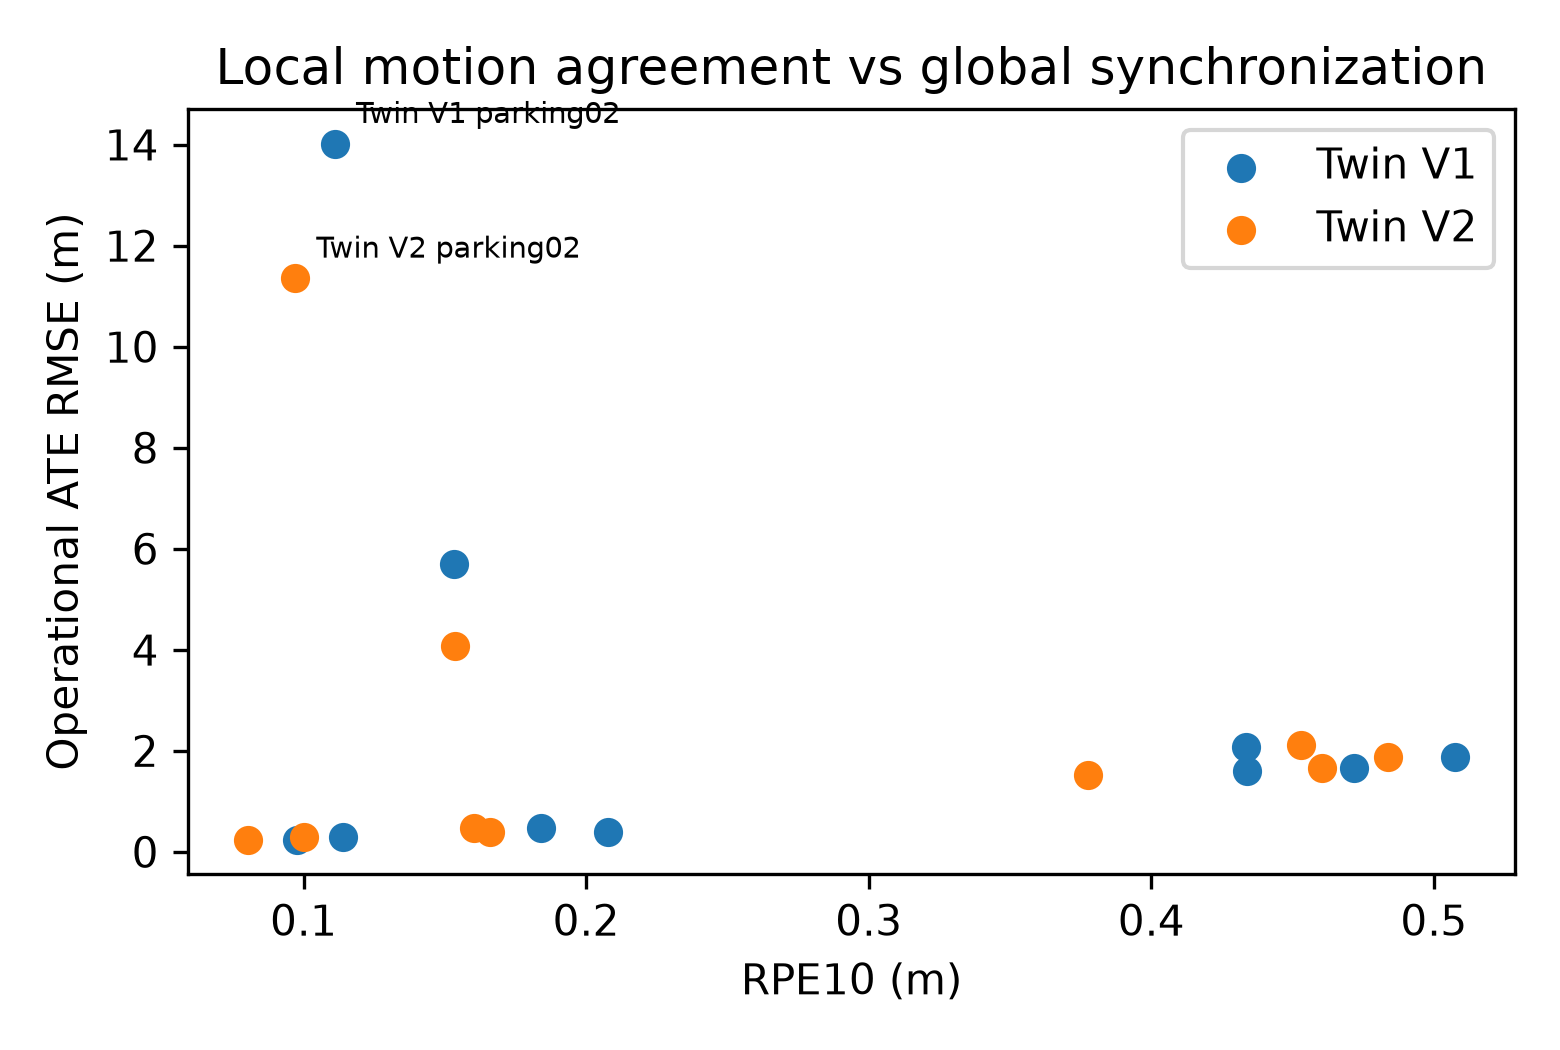
\includegraphics[width=.82\linewidth]{figures/v1_v2_local_vs_global_clean.png}
\caption{Frozen V1 and V2 comparison across local and global fidelity quantities. Model seeds are aggregated within each physical sequence.}
\end{figure}

\section{Local Versus Global Fidelity}
Across the ten i2Nav sequences, parking02 is the largest-divergence case: ATE 11.350 m, $D_p$ p95 22.345 m, and $D_\theta$ p95 $30.415^\circ$. Yet its RPE$_{10}$ is 0.097 m, the second smallest of ten. A median-split descriptive check identifies parking01 and parking02 as low-local/high-global cases.

At sequence level, persistent yaw mismatch and accumulated yaw residual have Pearson/Spearman associations 0.974/0.952. Heading divergence and position divergence have associations 0.988/0.952. The direct $I_\omega$--heading-divergence association is weaker (Pearson 0.381, Spearman $-0.030$), so the chain is a measured pathway rather than a universal monotonic law.

\begin{figure}[ht]\centering
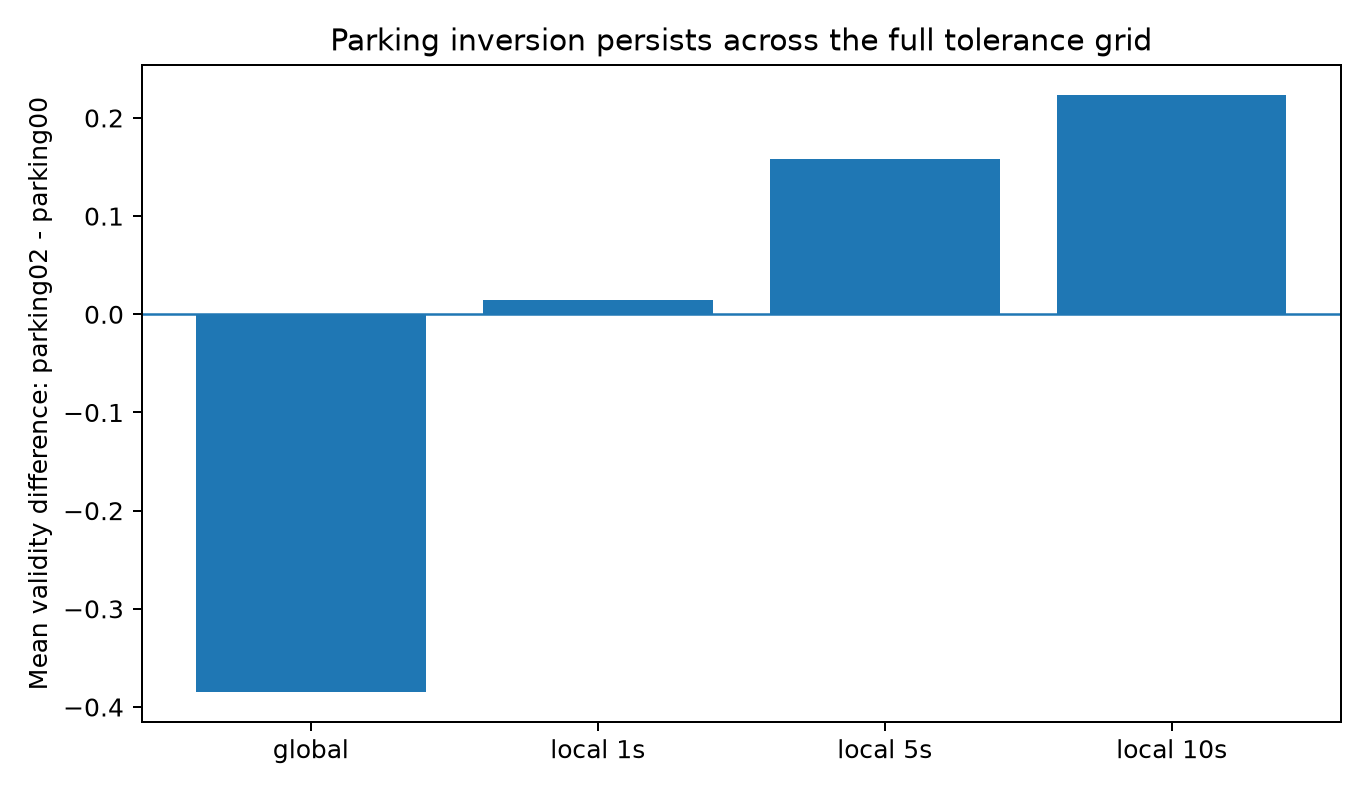
\includegraphics[width=.78\linewidth]{figures/e1_parking_full_grid_inversion.png}
\caption{parking00 and parking02 exchange ordering between global synchronization and finite-horizon local services over the prespecified tolerance grid.}
\end{figure}

\begin{figure}[ht]\centering
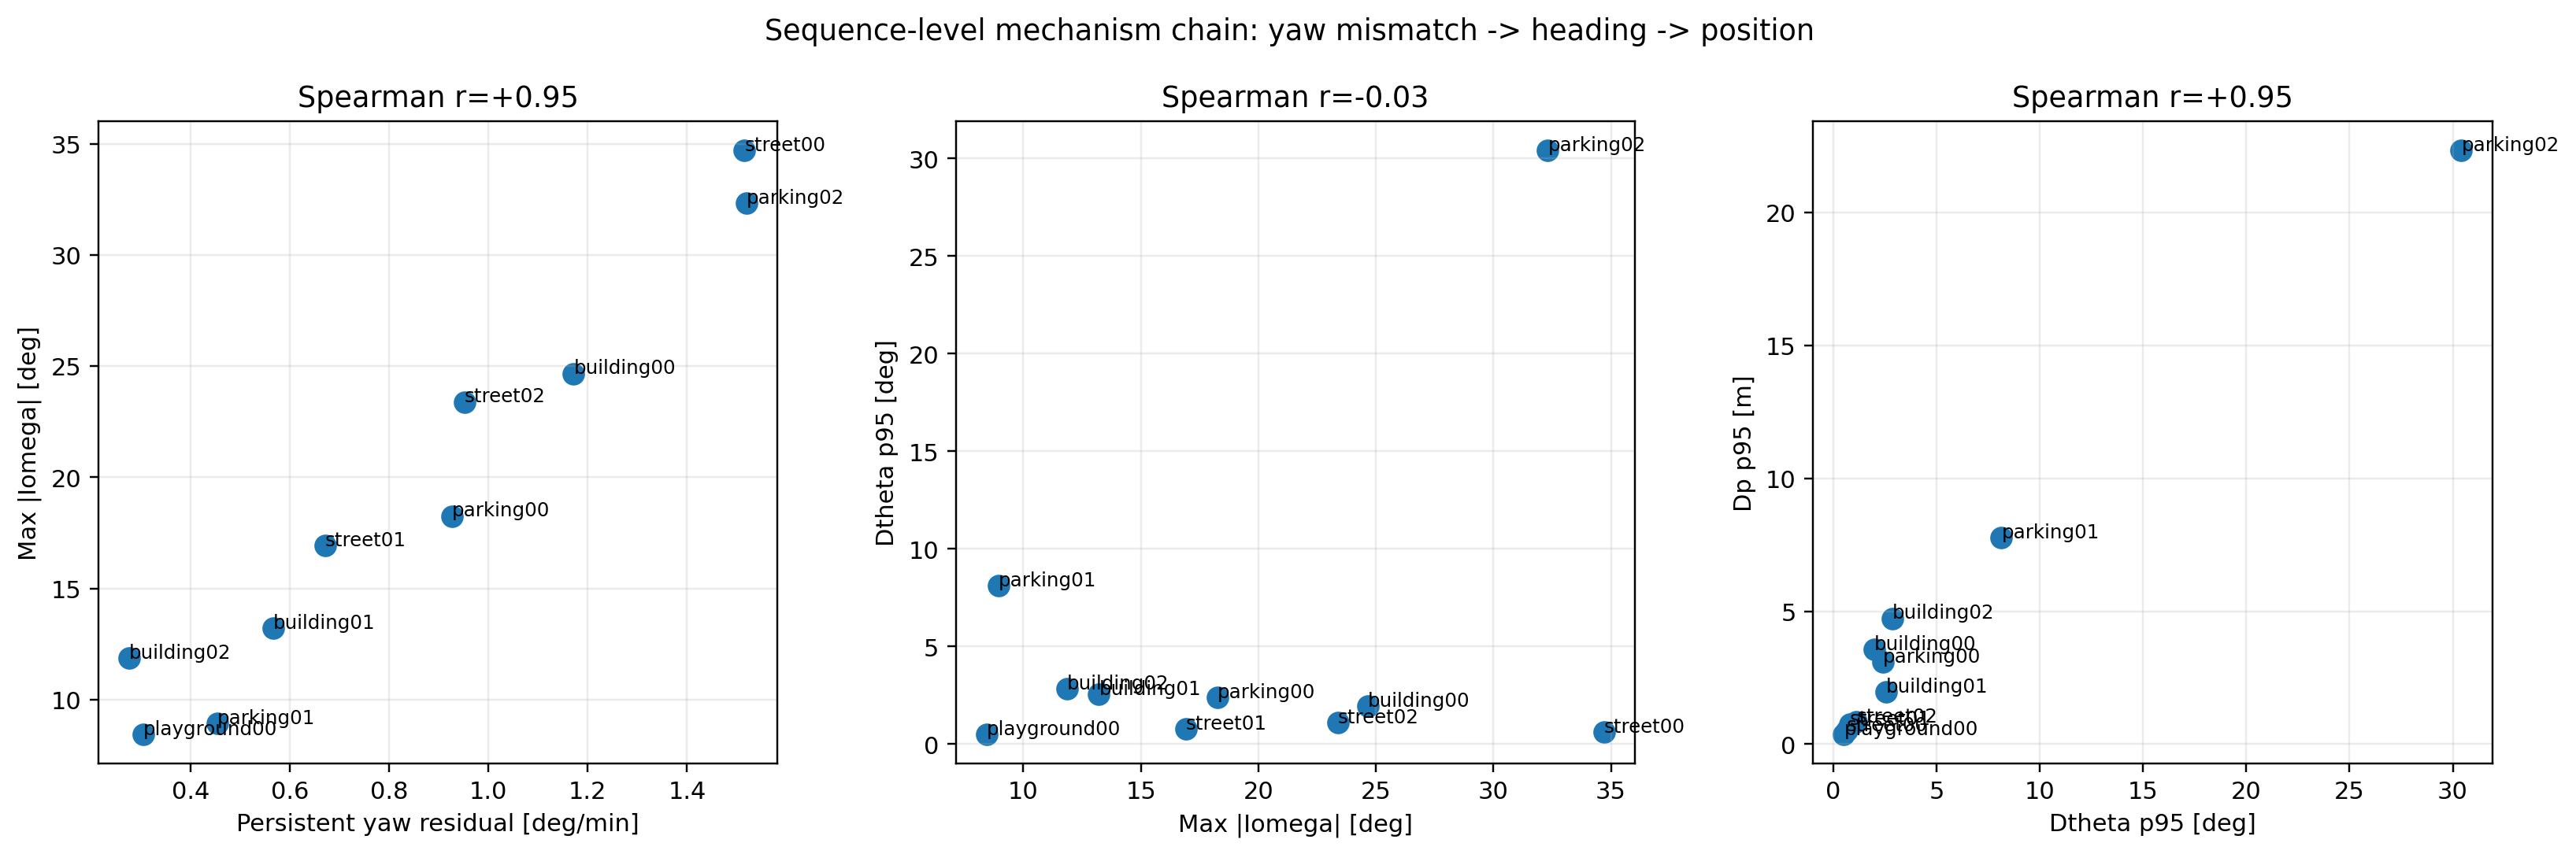
\includegraphics[width=.86\linewidth]{figures/persistent_yaw_mechanism.png}
\caption{Persistent yaw mismatch, accumulated yaw residual, heading divergence, and position divergence across the frozen i2Nav sequences.}
\end{figure}

\begin{figure}[ht]\centering
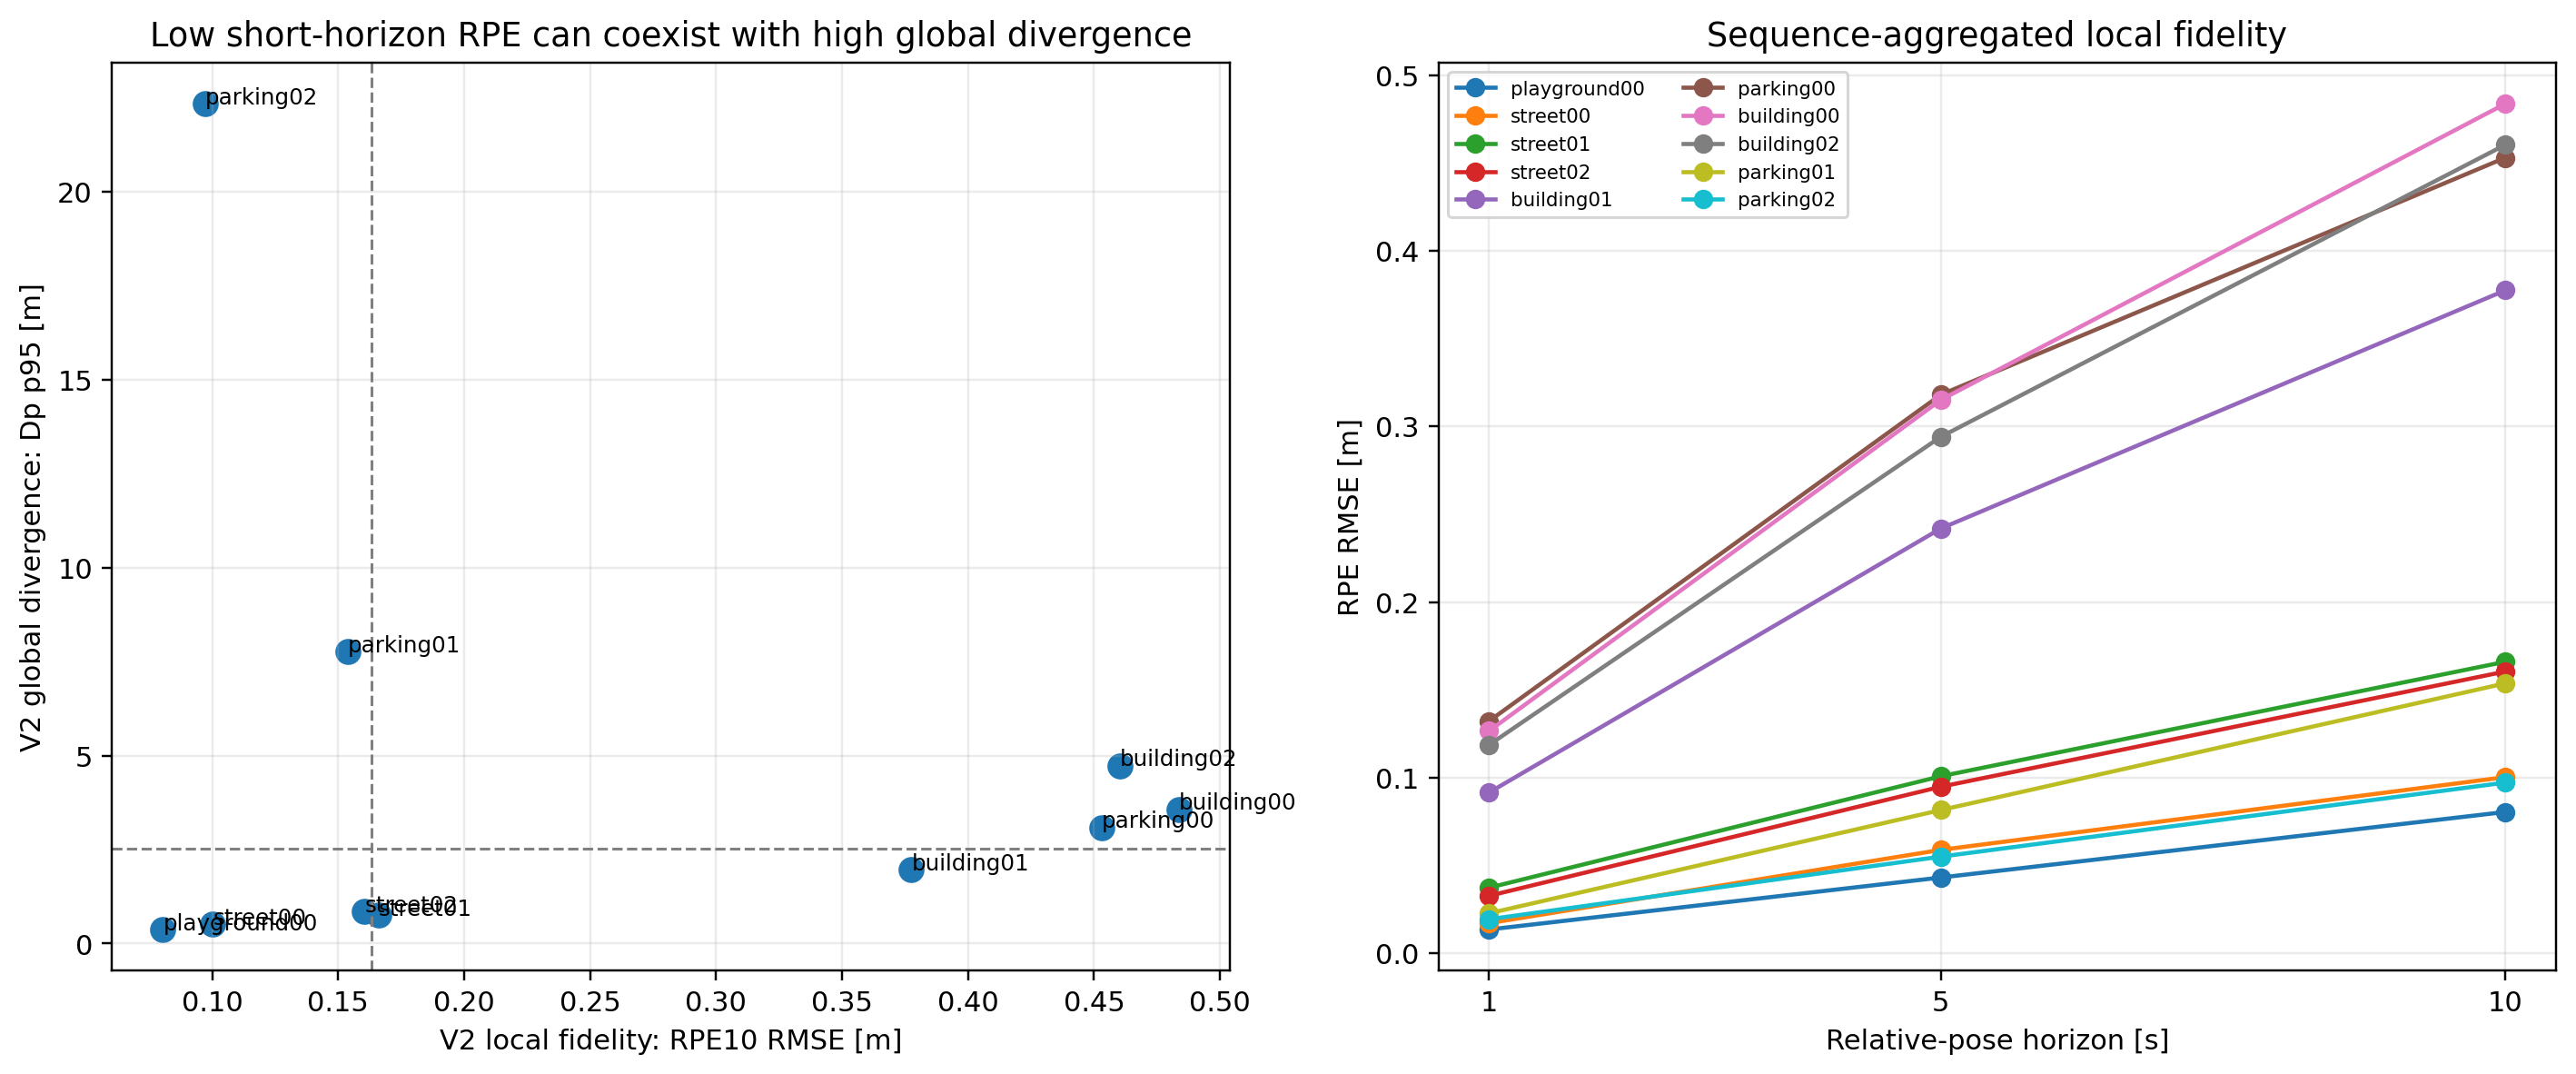
\includegraphics[width=.80\linewidth]{figures/local_vs_global_fidelity.png}
\caption{All-sequence comparison of finite-horizon local error and accumulated global physical--virtual divergence.}
\end{figure}

\section{Condition-Dependent Fidelity}
Condition bins were frozen from condition variables rather than outcomes. High wheel--IMU disagreement worsens RPE$_1$ in 10/10 sequences with median increase 0.005 m. High turning worsens RPE$_5$ and RPE$_{10}$ in 9/10 sequences, with median increases 0.018 and 0.026 m. High acceleration worsens $D_p$ p95 in 9/10 sequences by a median 0.024 m, while high curvature worsens $D_\theta$ p95 in 10/10 by a median $0.278^\circ$. These within-sequence contrasts are smaller than the between-sequence spread but recur consistently.

parking02 remains the highest-divergence sequence inside high speed, acceleration, turning, curvature, and wheel--IMU-disagreement bins. No single measured condition explains the complete sequence-level failure.

\begin{figure}[ht]\centering
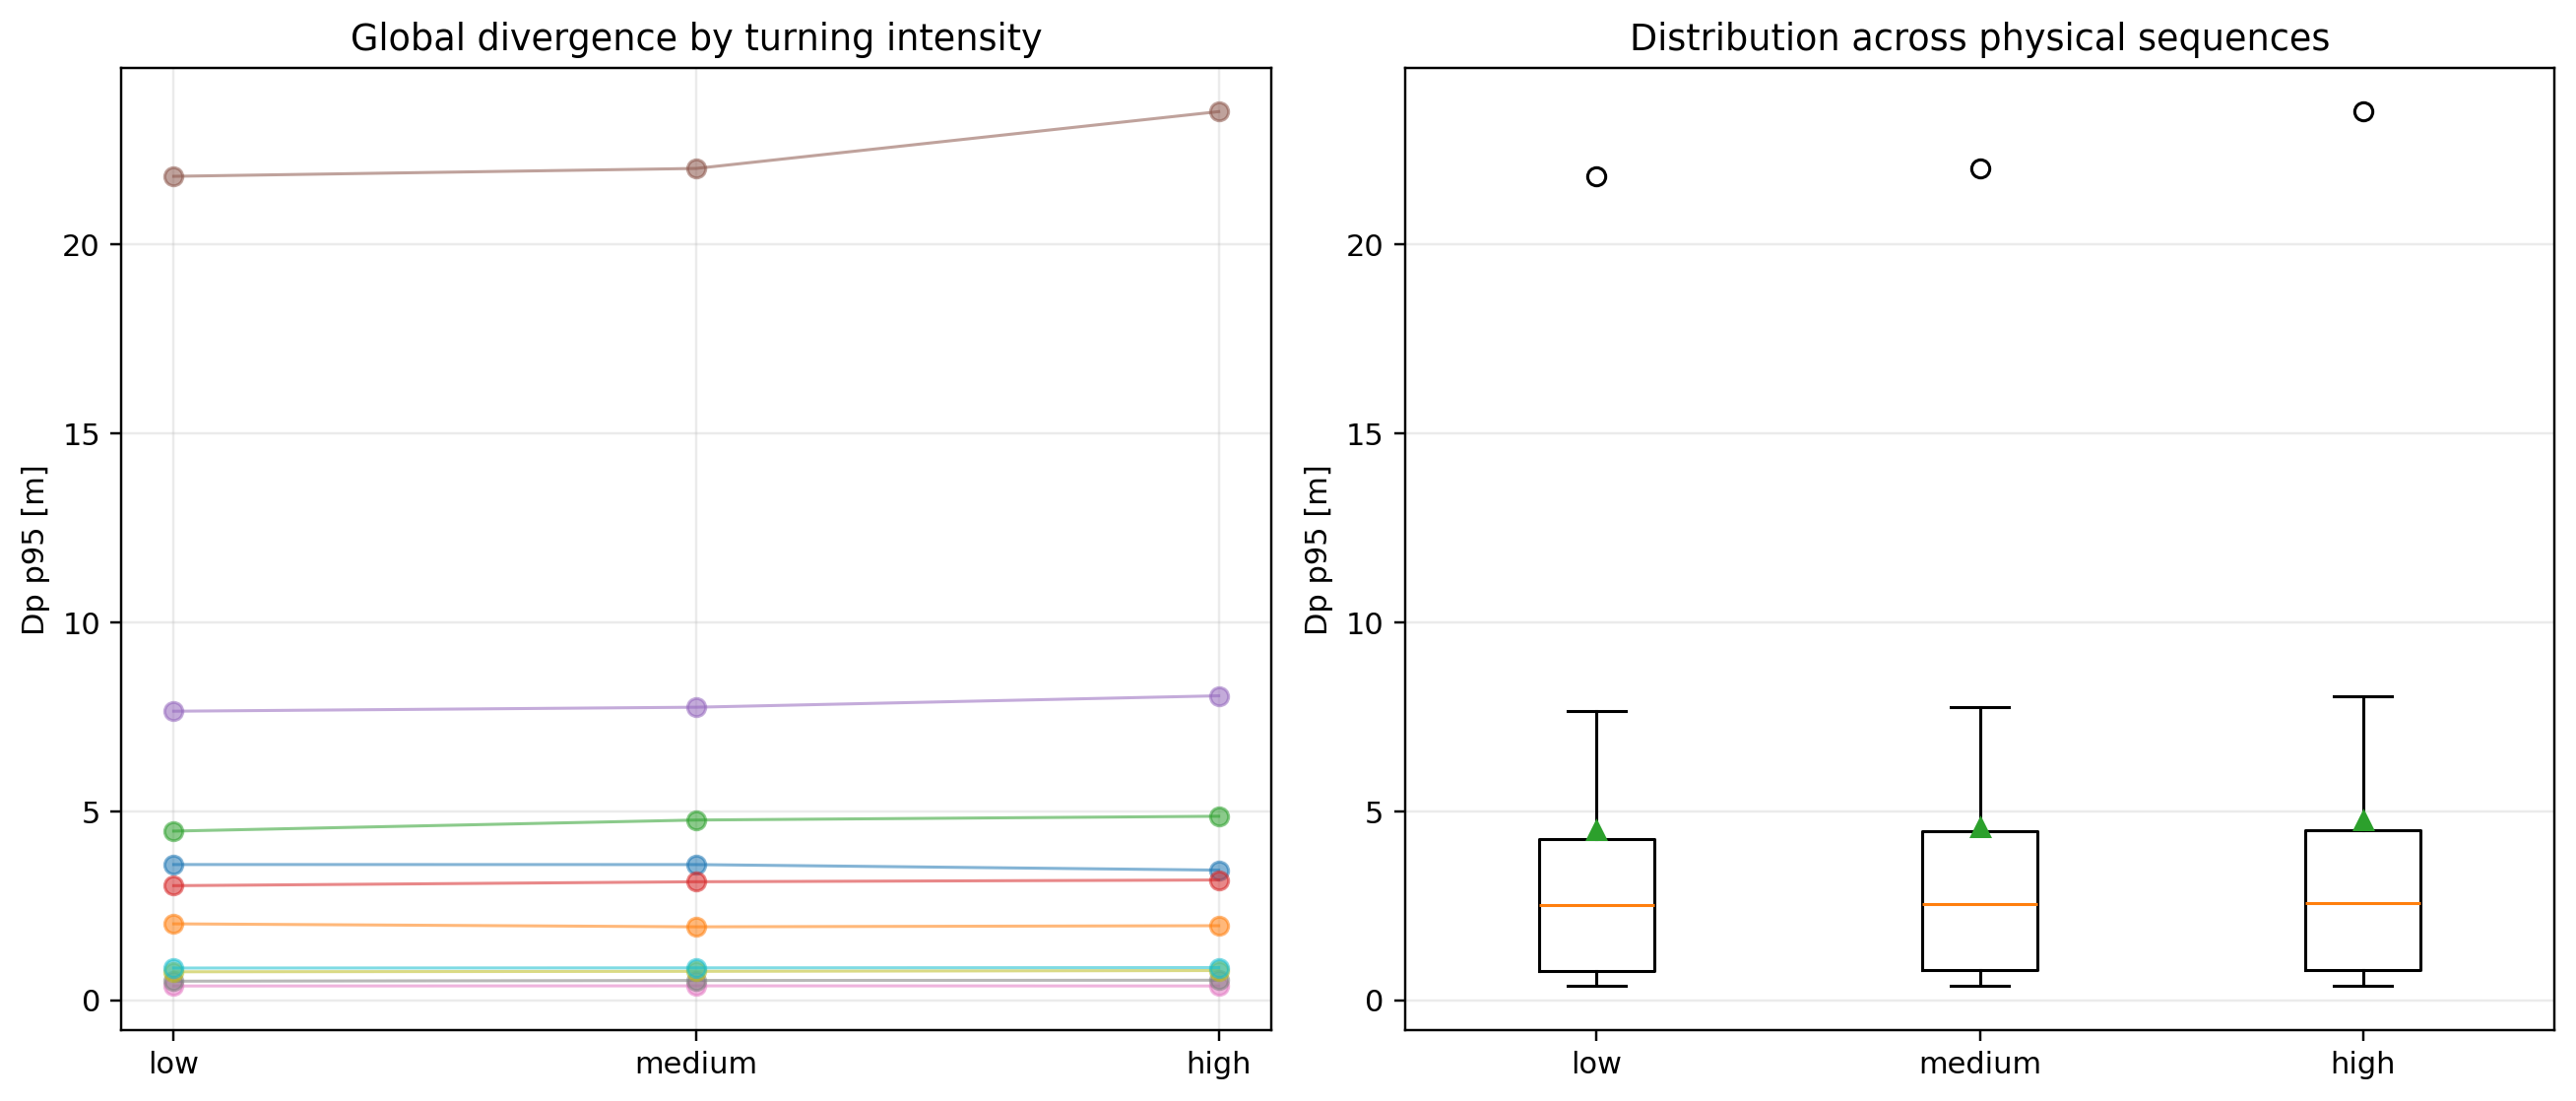
\includegraphics[width=.86\linewidth]{figures/condition_dependent_fidelity.png}
\caption{Condition-dependent changes in local and global fidelity after within-run calculation and seed aggregation within physical sequence.}
\end{figure}

\section{Benign Fidelity Distributions and Held-Out Envelope Validation}
The empirical Twin Fidelity Profile stores ATE, heading MAE, RPE$_1$, RPE$_5$, RPE$_{10}$, persistent yaw mismatch, $I_\omega$, and $D_p/D_\theta$ tail quantities for every frozen run. The descriptive p95 envelope changes materially with context. For example, elapsed-time-conditioned $D_p$ p95 rises from 5.828 m in the early bin to 17.118 m in the late bin.

Leave-one-sequence-out p95 sensitivity is lower for $D_v$ (median relative sensitivity 0.078), $I_\omega$ (0.118), and $D_\omega$ (0.184) than for $D_p$ (0.587) and $D_\theta$ (0.704). Removing parking01 and parking02 lowers late-bin $D_p$ p95 from 17.118 to 4.510 m. The envelope is therefore stable enough for descriptive rate-domain characterization but strongly sequence-dependent in accumulated position and heading.

Held-out conditioned and unconditional coverage are similar in the current ten-sequence data. Condition dependence is evident in envelope width and fidelity distributions, but conditioning has not established a uniformly superior held-out predictor.

\begin{figure}[ht]\centering
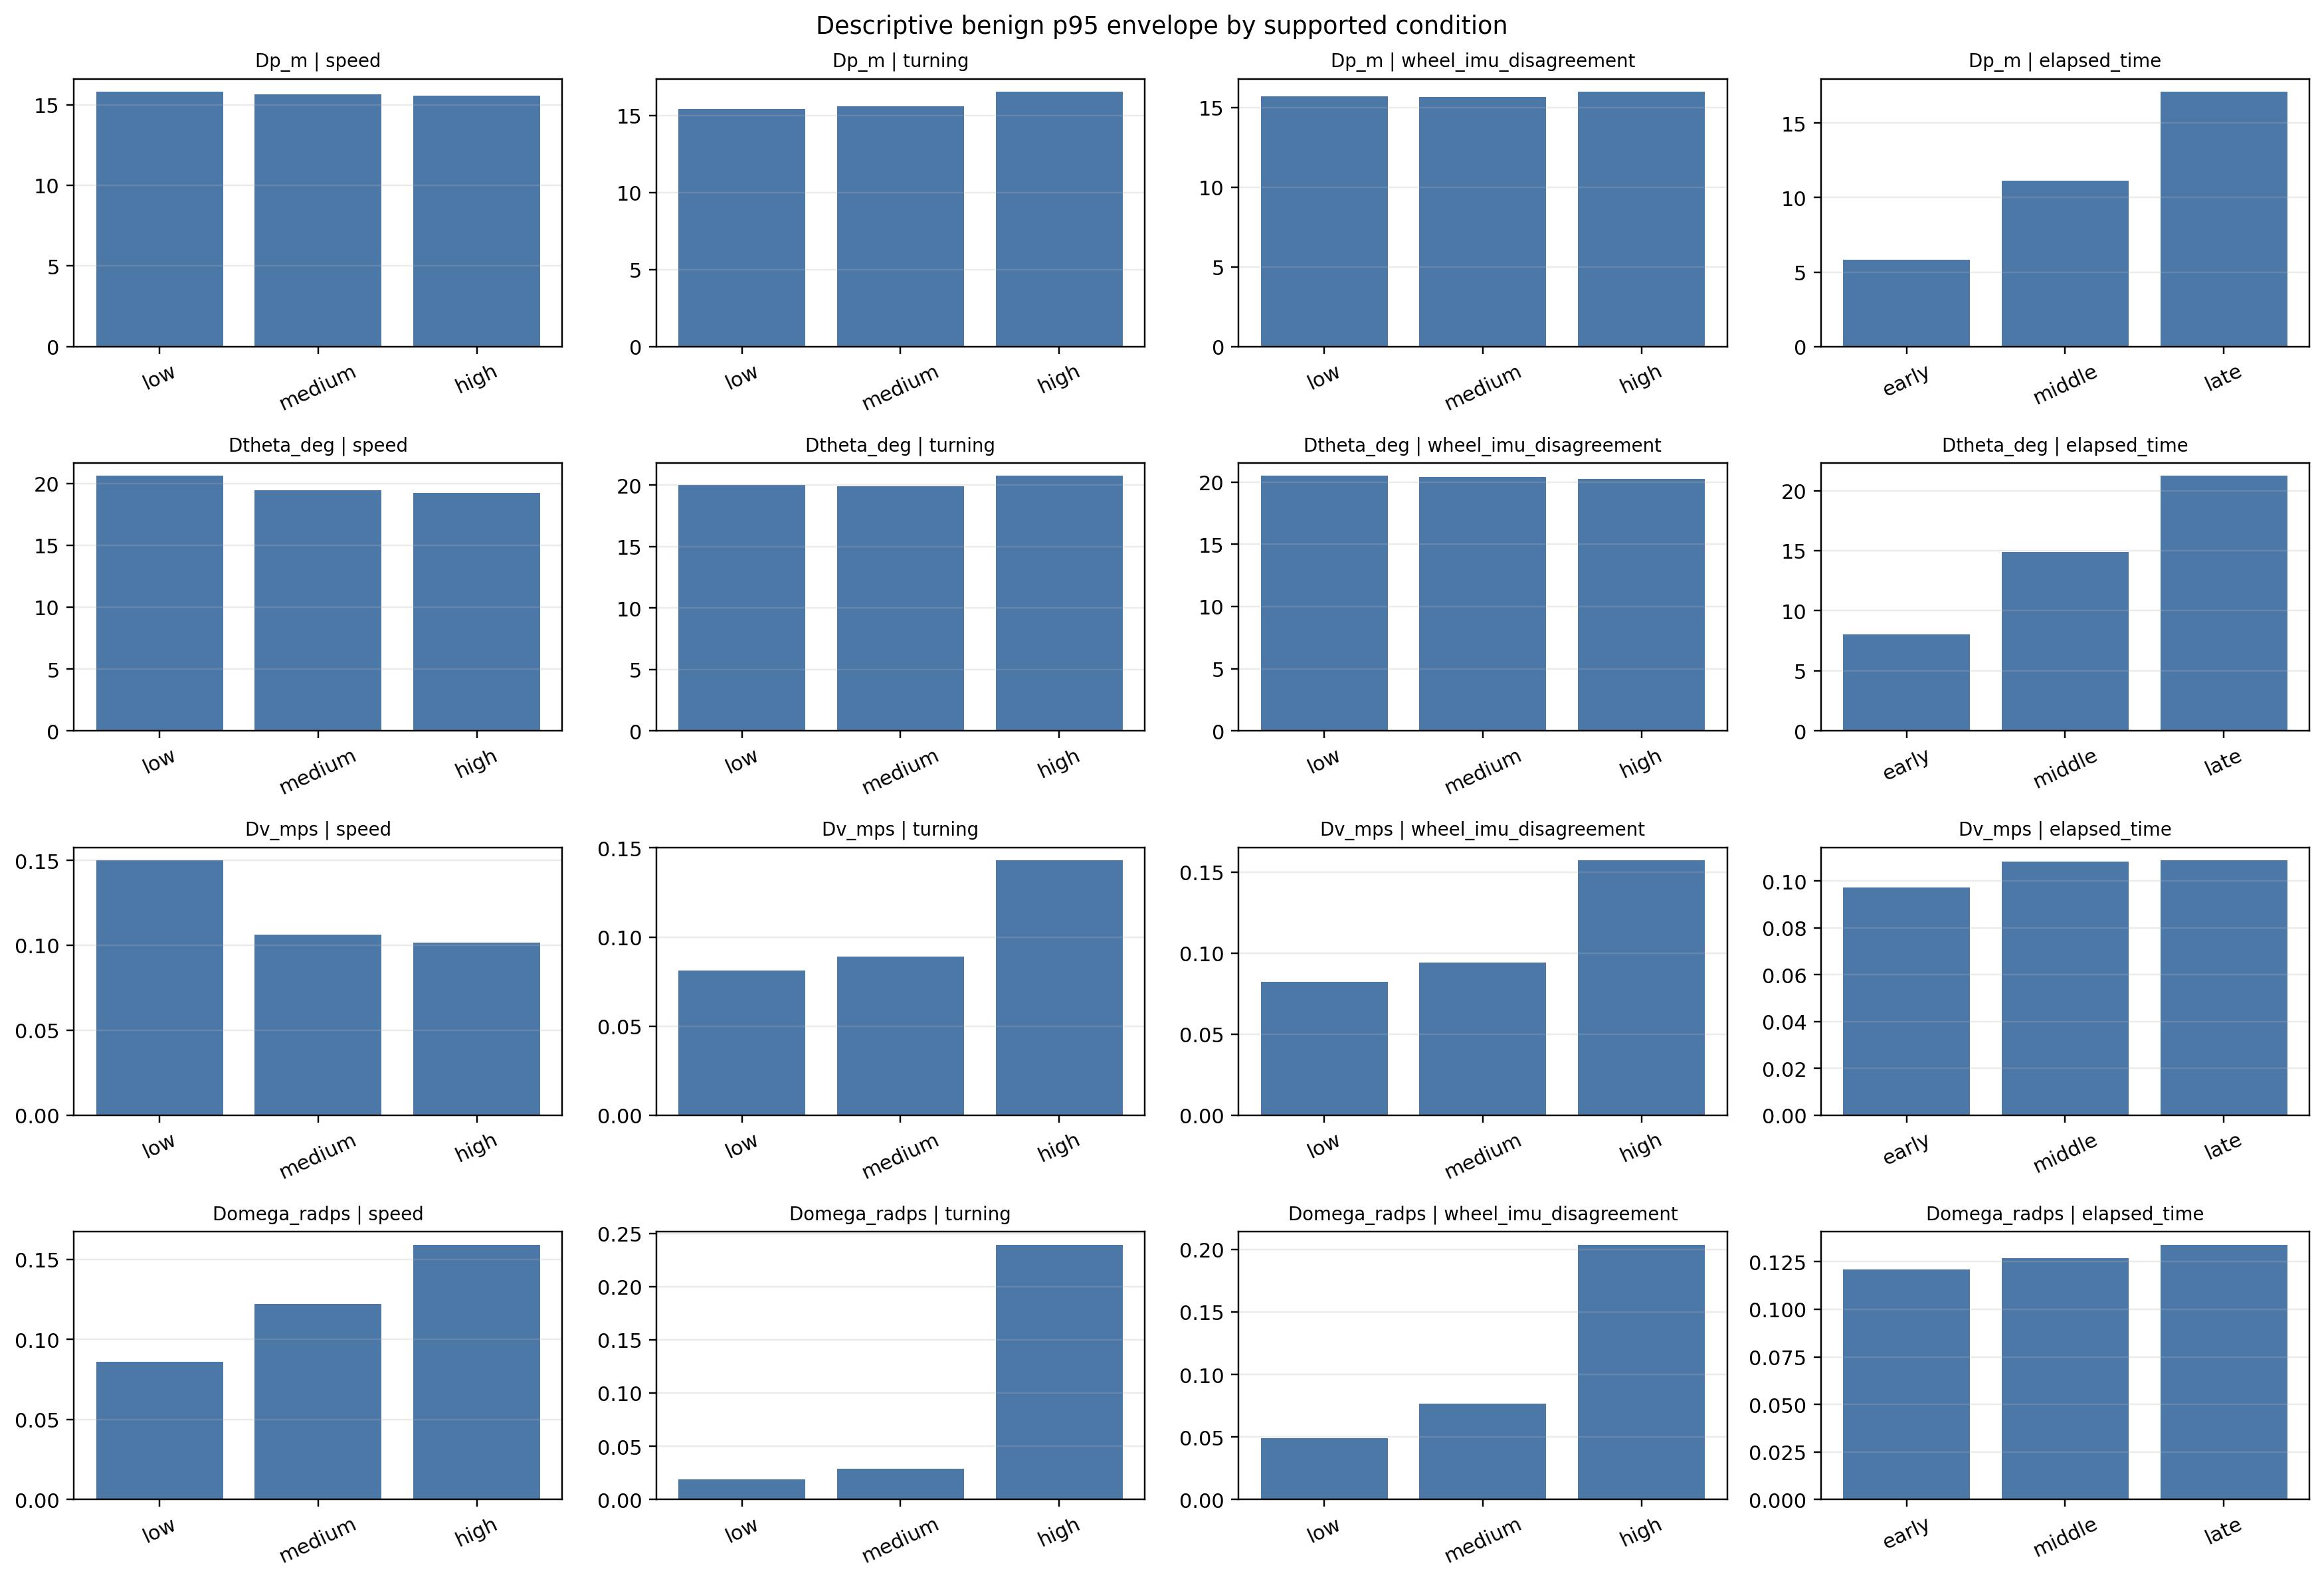
\includegraphics[width=.84\linewidth]{figures/benign_envelope_by_condition.png}
\caption{Componentwise benign p95 summaries across supported operating contexts. These are descriptive percentiles rather than detection thresholds.}
\end{figure}

\begin{figure}[ht]\centering
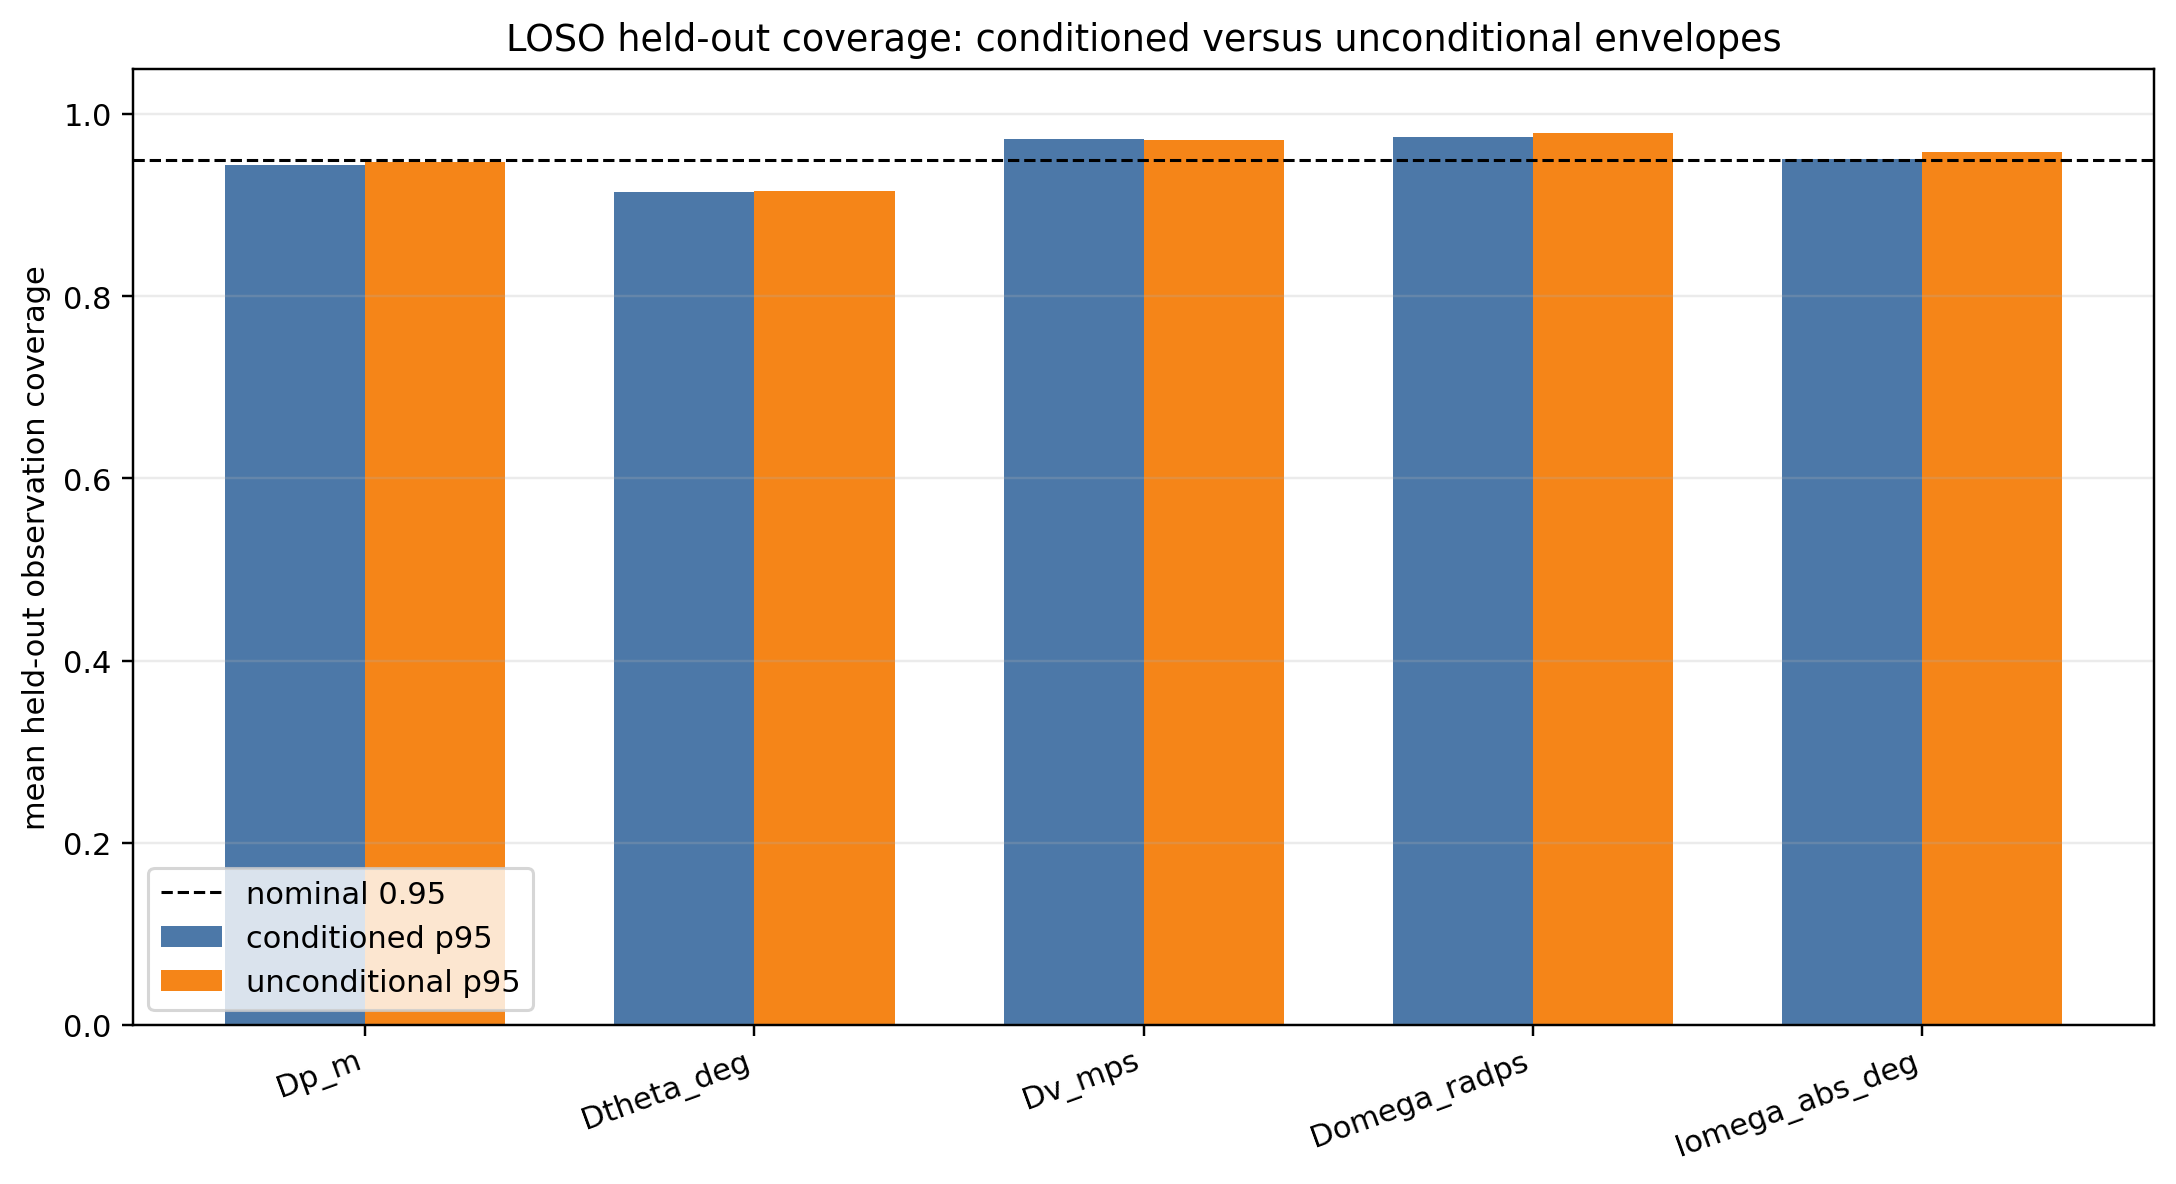
\includegraphics[width=.84\linewidth]{figures/loso_envelope_coverage.png}
\caption{Leave-one-physical-sequence-out coverage of conditioned and unconditional descriptive envelopes.}
\end{figure}

\section{Official i2Nav Benchmark}
The separate official-protocol evaluation exports frozen trajectories in TUM format, converts the internal ENU/FLU representation to the i2Nav NED convention, associates timestamps within 0.005 s, applies SE(3) alignment without scale correction, and reports APE and distance-based RPE.

Frozen V2 achieves macro APE translation RMSE 1.635 m, APE rotation RMSE $3.011^\circ$, RPE$_{50\mathrm{m}}$ 1.310 m, RPE$_{100\mathrm{m}}$ 2.217 m, and RPE$_{300\mathrm{m}}$ 3.635 m. Fixed physics has macro APE 3.299 m, so V2 reduces the macro mean by 50.441\%; the mean of sequence-wise relative reductions is 34.894\%. V2 improves APE on 9/10 sequences with sequence-level bootstrap interval $[-3.492,-0.279]$ m and sign-flip $p=0.0059$. Alignment compresses some accumulated drift, so these benchmark numbers remain separate from unaligned physical--virtual fidelity.

\begin{figure}[ht]\centering
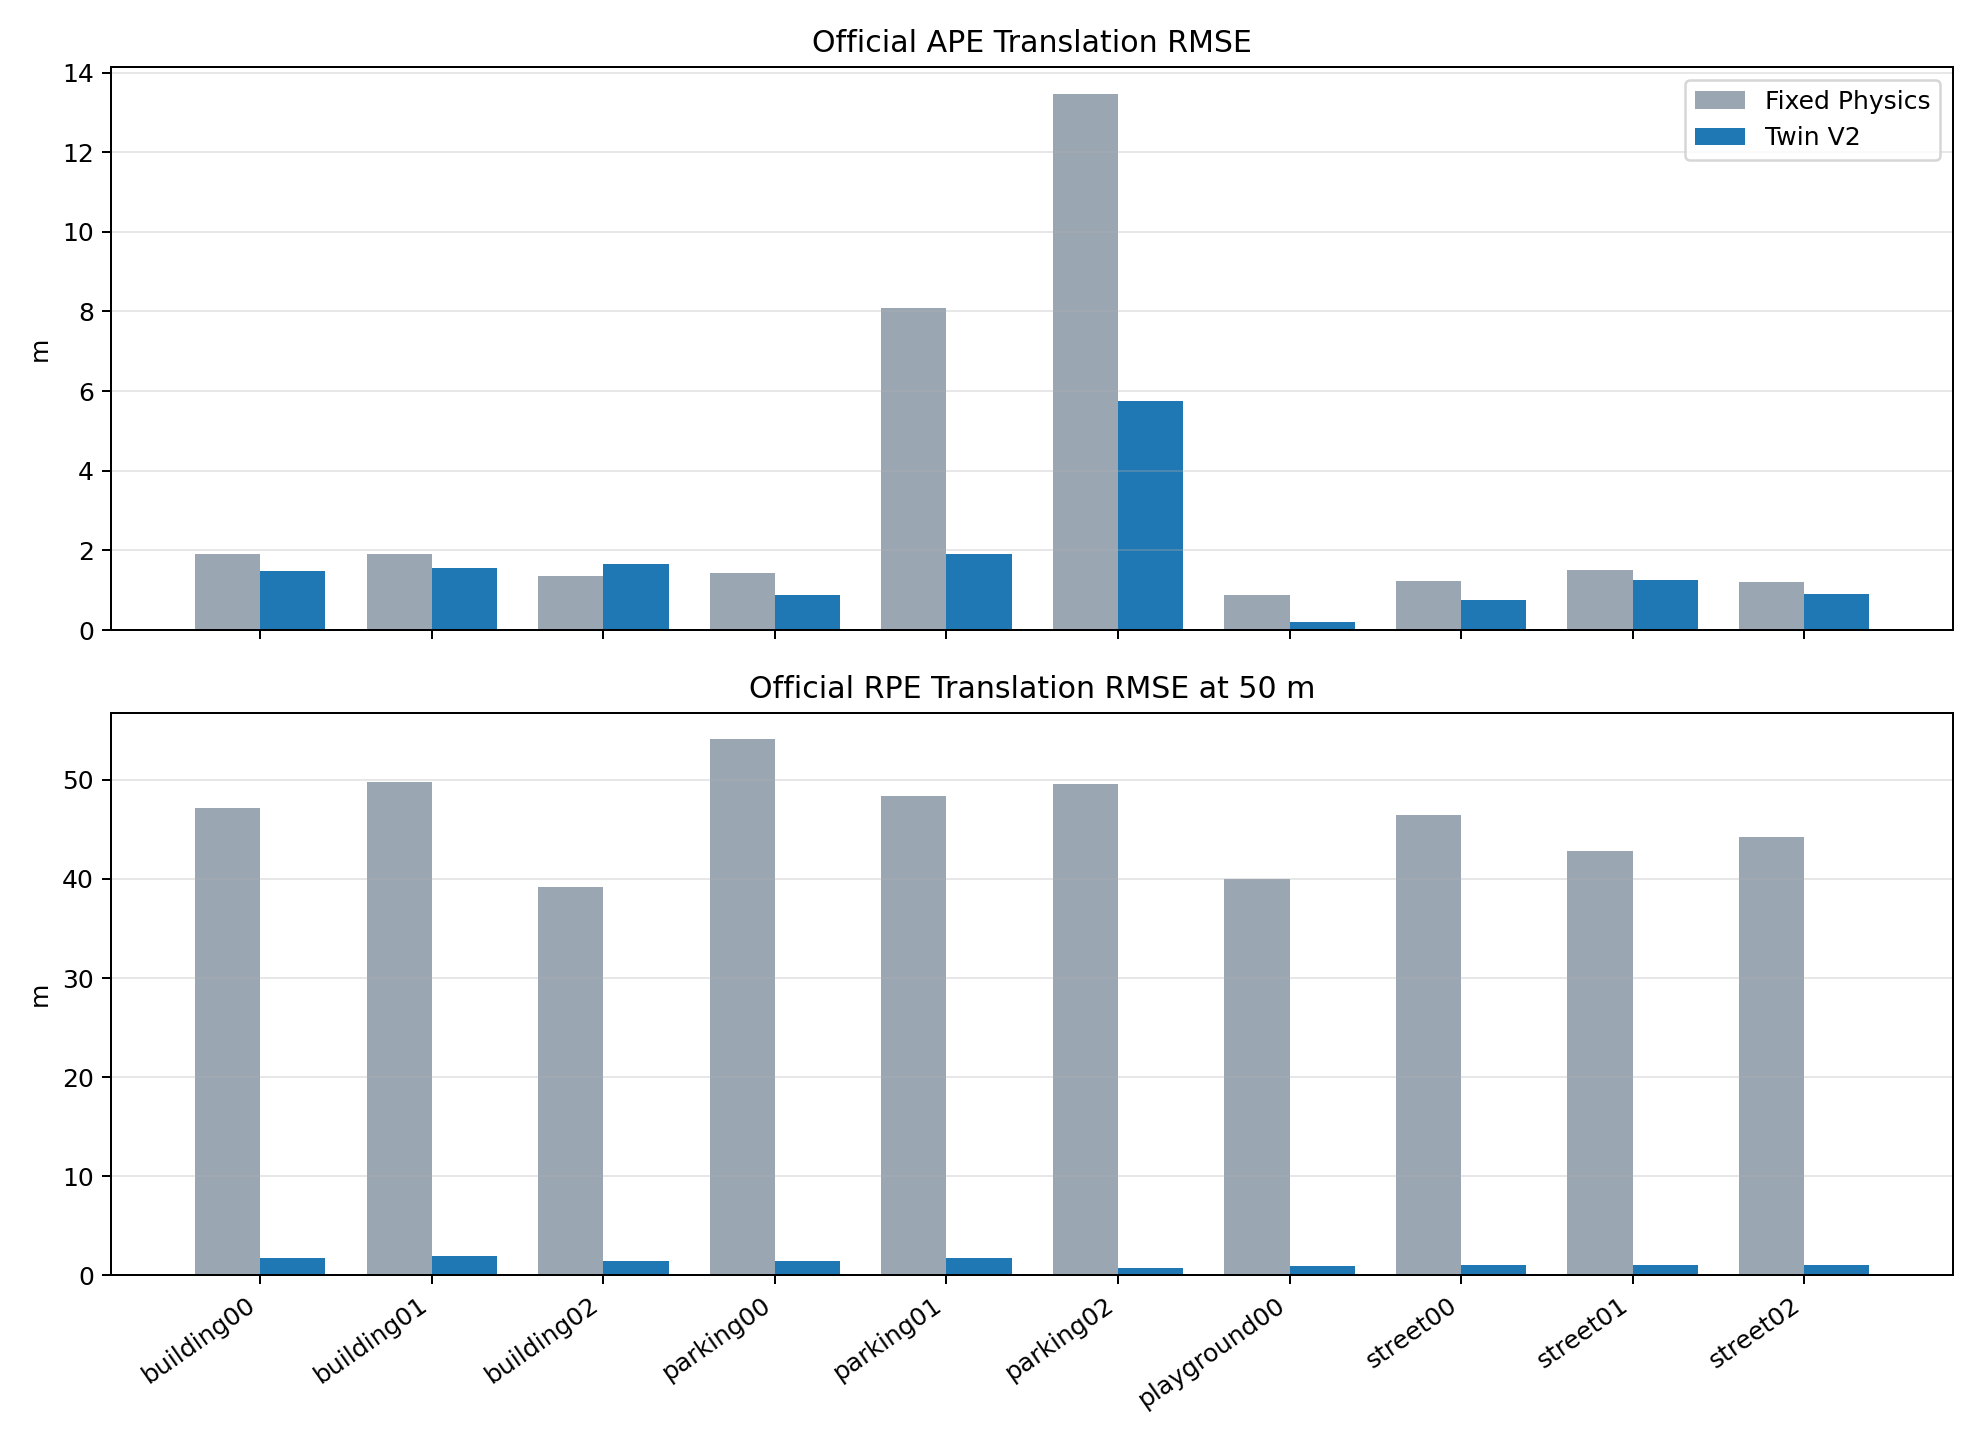
\includegraphics[width=.84\linewidth]{figures/official_benchmark_results.png}
\caption{Official-protocol frozen V2 and fixed-physics i2Nav benchmark results. Internal unaligned fidelity is evaluated separately.}
\end{figure}

\section{Service-Relative Rank Experiments}
The E1 tolerance-grid study compares sequence ordering under global and finite-horizon services. parking00 wins all 36 global tolerance points, whereas parking02 wins all 25 local points at each of 1, 5, and 10 s. Median Kendall association of global pass rate is 0.708 with ATE and 0.151 with RPE$_{10}$; local-10-s pass rate has association 0.762 with RPE$_{10}$ and 0.333 with ATE. The result shows that metric choice changes service decisions.

The condition-aware online support envelope improves on its unconditional comparator at 23/111 comparable grid points and ties at 88/111. A nested service-risk estimator also does not beat the required simpler baselines. These are completed negative results.

\begin{figure}[ht]\centering
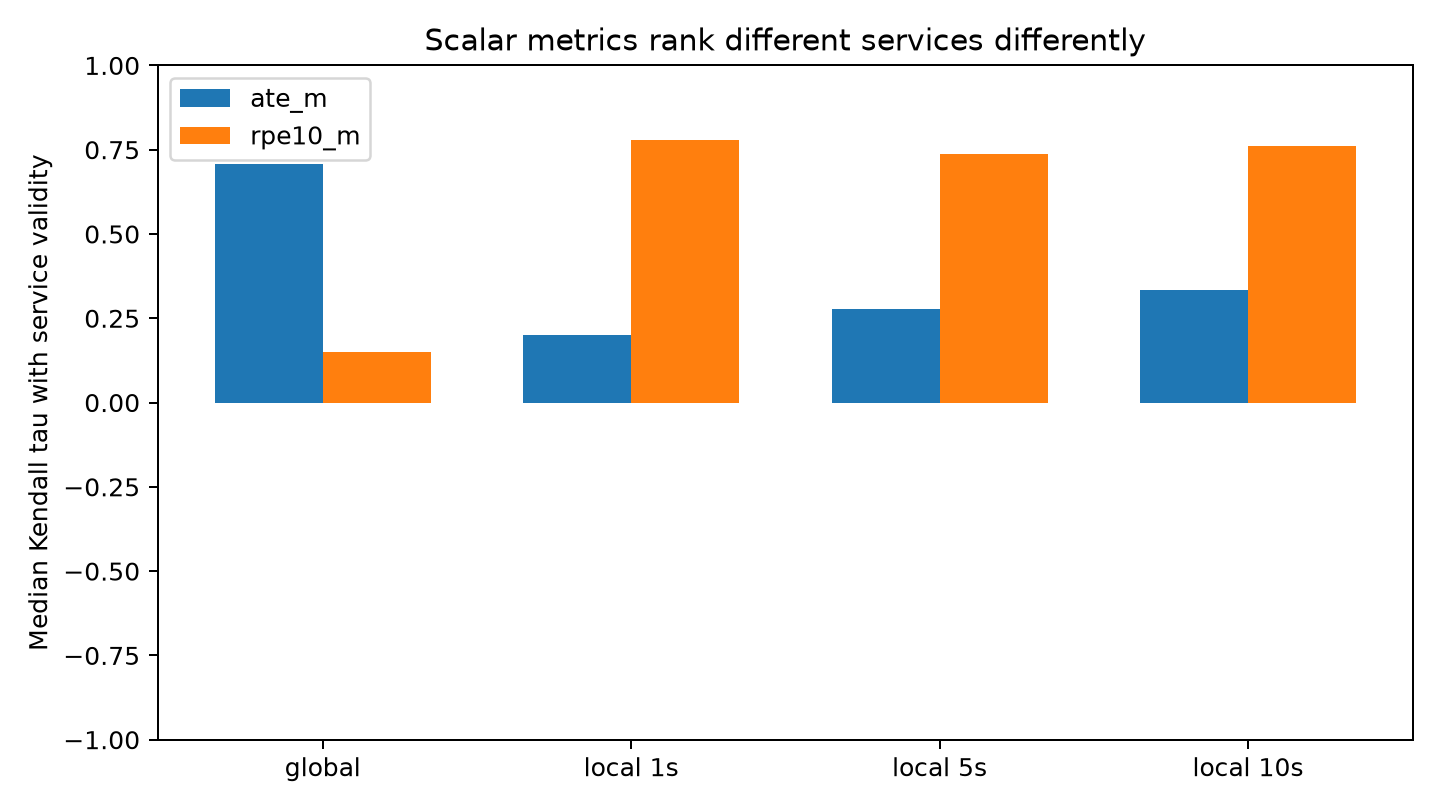
\includegraphics[width=.80\linewidth]{figures/e1_metric_service_rank_alignment.png}
\caption{Association of global and finite-horizon service validity with ATE and horizon-matched RPE.}
\end{figure}

\section{Sampled-Delivery Timing Study}
The completed historical timing study evaluates four services over twenty nominal delivery settings, producing 800 sequence--service--cell outcomes nested within ten physical sequences. Mean joint satisfaction at ideal 10-Hz/0-ms delivery is 0.985, 0.949, 0.960, and 0.503 for local 1-s, local 5-s, local 10-s, and global services. At 2 Hz/200 ms it is 0.712, 0.657, 0.730, and 0.445. At that operating point freshness satisfaction is 1.000 under the specified limits, so remaining qualification failures arise from physical discrepancy.

On the saved 10-Hz state clock, nominal 25- and 50-ms delays select identical represented histories. Integer-clock analysis yields three distinct histories across the five nominal delays for each rate/phase group. At 5 Hz, however, 0 and 50 ms select different histories in all 30 phase-zero V2 runs.

\begin{figure}[ht]\centering
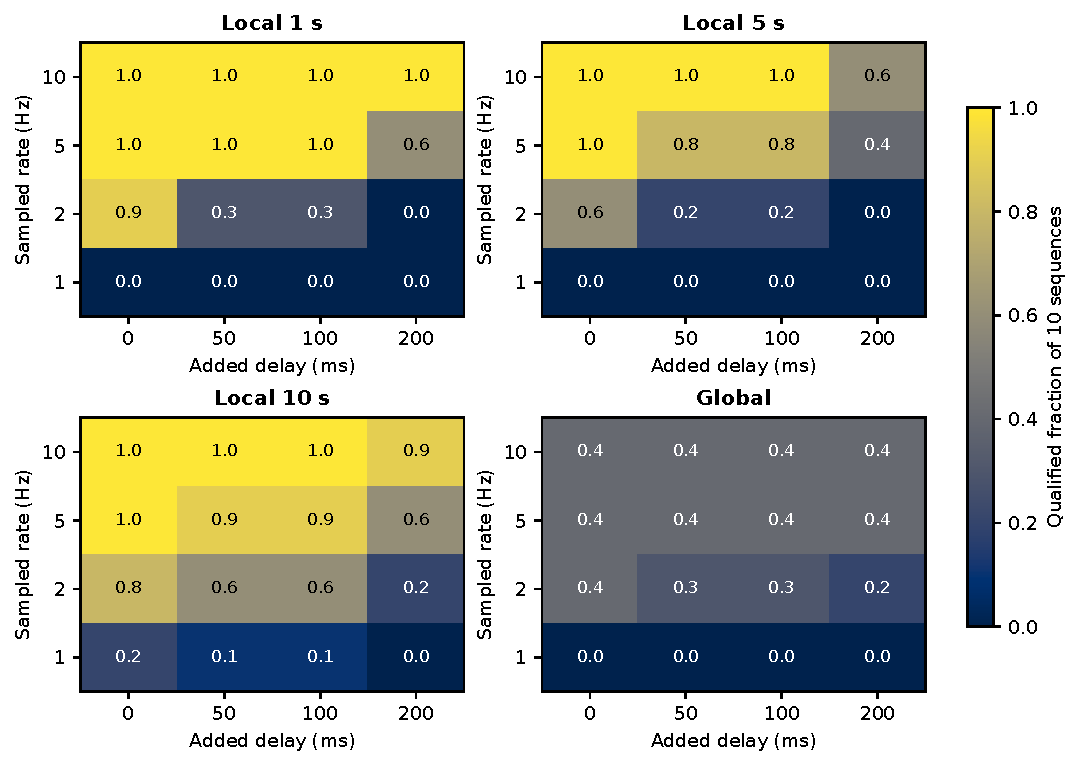
\includegraphics[width=.90\linewidth]{figures/cross_sequence_qualification_surfaces.pdf}
\caption{Historical four-service qualification surfaces. The 25-ms column is omitted because it aliases 50 ms on the saved state clock.}
\end{figure}

\section{Qualification Transfer and Comparator Checks}
The qualification-label holdout fits a cell-specific empirical surface on nine sequences and evaluates the remaining sequence. At the reported pooled operating point, the empirical surface accepts 235/800 cells and falsely qualifies 5/235 (2.1\%). Service identity accepts 200/800 and falsely qualifies 75/200 (37.5\%). The sequence-bootstrap difference is $-35.4$ percentage points with interval $[-44.4,-25.1]$. AoI-only has 60 false qualifications among 250 accepted cells, adapted kinematic staleness 97/242, and motion logistic 56/235. The empirical-versus-logistic paired interval crosses zero.

These numbers are historical qualification-label-held-out results. They do not provide end-to-end outer-sequence exclusion because checkpoints used to generate some of the other nine qualification trajectories could include the outer sequence upstream. The doubly nested experiment in Appendix~\ref{app:pending} is designed to replace these counts.

\begin{figure}[ht]\centering
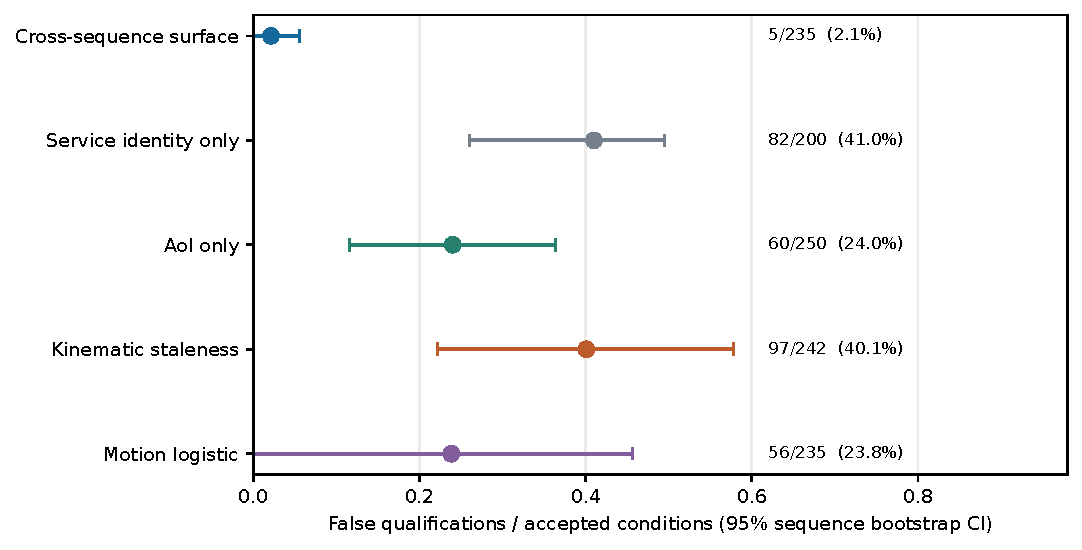
\includegraphics[width=.84\linewidth]{figures/heldout_qualification_comparison.pdf}
\caption{Historical pooled qualification operating points with physical-sequence bootstrap intervals and explicit false/accepted denominators.}
\end{figure}

\begin{figure}[ht]\centering
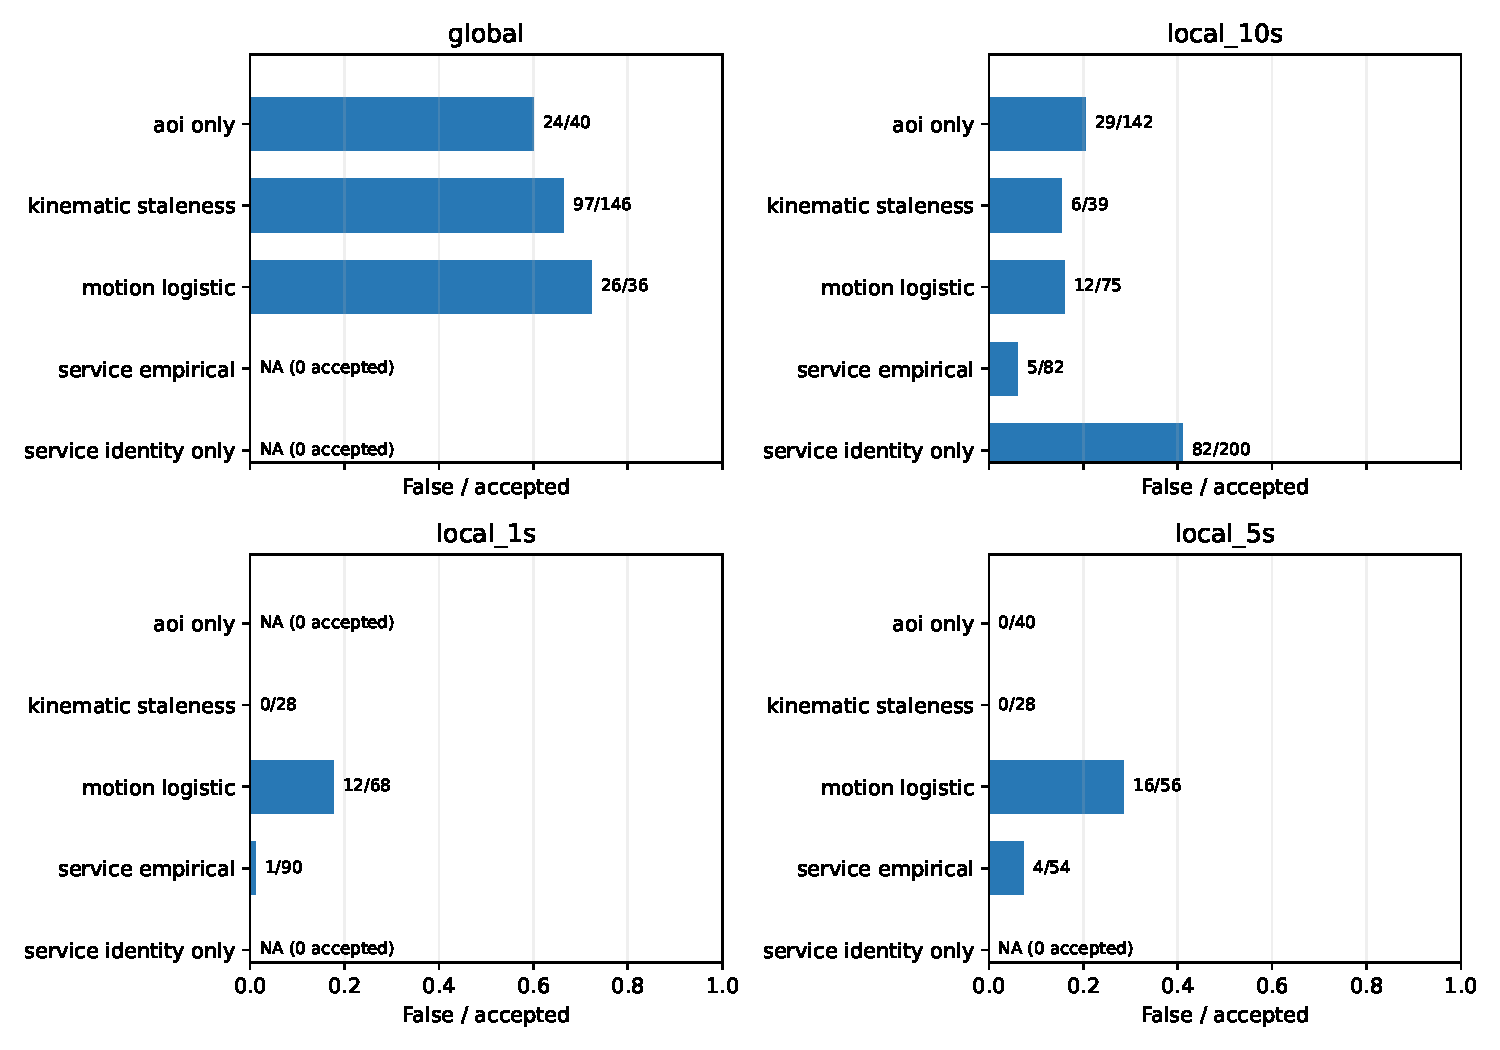
\includegraphics[width=.80\linewidth]{figures/per_service_qualification.pdf}
\caption{Per-service accepted-cell and false-qualification counts. Comparator acceptance differs within services.}
\end{figure}

\begin{figure}[ht]\centering
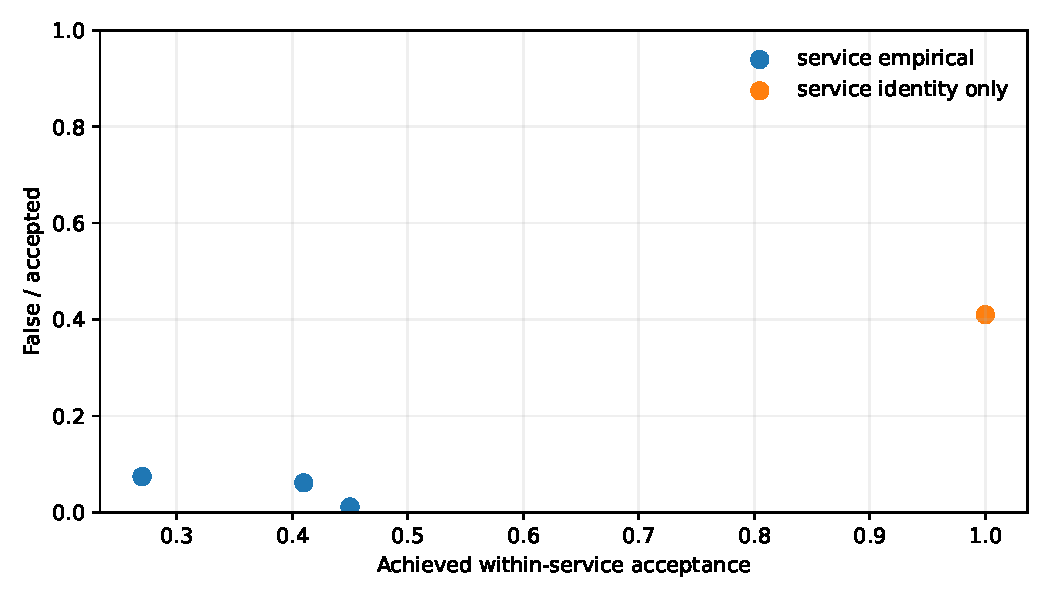
\includegraphics[width=.80\linewidth]{figures/surface_vs_identity.pdf}
\caption{Per-service surface and service-identity operating points. The identity score is tied across each service's delivery cells.}
\end{figure}

\section{Remediability Ledger and Frozen-Configuration Sensitivity}
At 2 Hz/200 ms, the historical 40-case ledger contains 30 delivery-remediable, six persistent, and four already-qualified sequence--service cases. The predeclared 5-Hz/50-ms sampled configuration restores 27/30 remediable cases. All 30 remediable cases are discrepancy-only at this operating point because the evaluated freshness requirement is met. Requirements 0.70, 0.80, and 0.90 yield partitions 17/5/18, 30/6/4, and 29/9/2, respectively.

A deterministic fixed-physics alternate yields 23 remediable, 16 persistent, and one already-qualified case. V2 leaves six persistent cases rather than 16 and is the only one of the two configurations with global cases that become remediable. The exact partition is therefore model- and threshold-dependent, while the distinction between delivery and model discrepancy remains computable.

\begin{figure}[ht]\centering
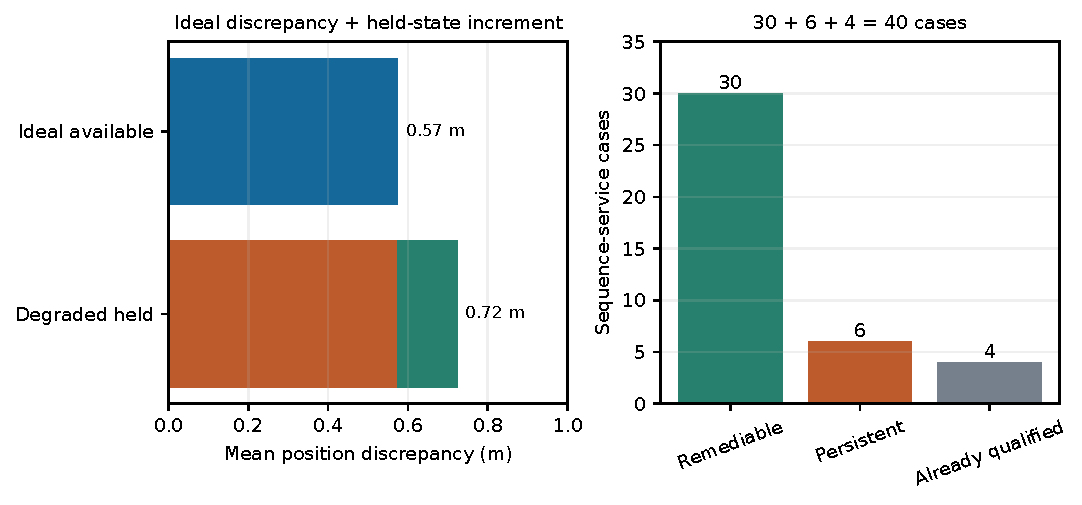
\includegraphics[width=.88\linewidth]{figures/held_state_mechanism_and_remediability.pdf}
\caption{Historical ideal-state discrepancy, held-state increment, and complete sequence--service case accounting.}
\end{figure}

\begin{figure}[ht]\centering
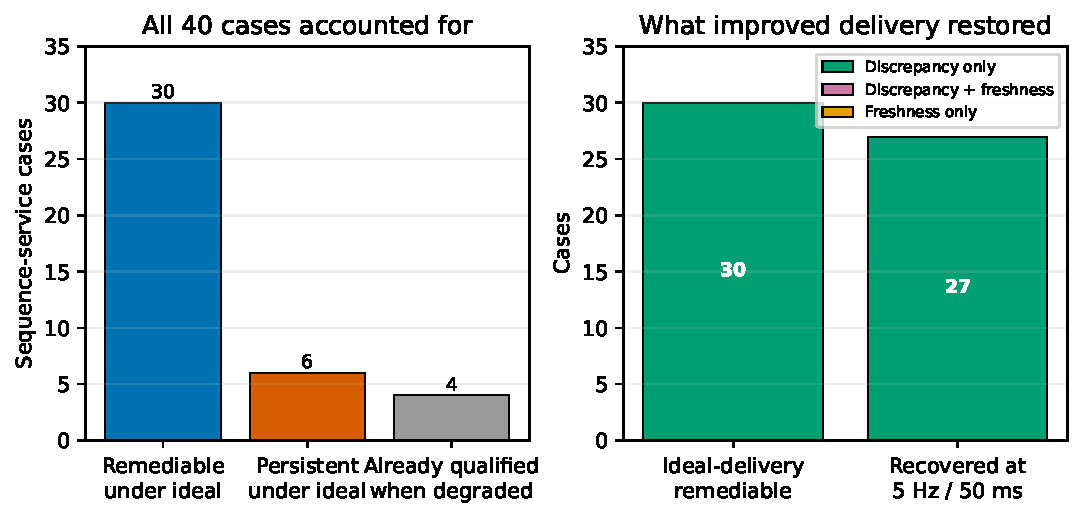
\includegraphics[width=.84\linewidth]{figures/delivery_recovery_decomposition.pdf}
\caption{Failure-component decomposition of the historical 30/6/4 ledger and the 27 practical recoveries.}
\end{figure}

\begin{figure}[ht]\centering
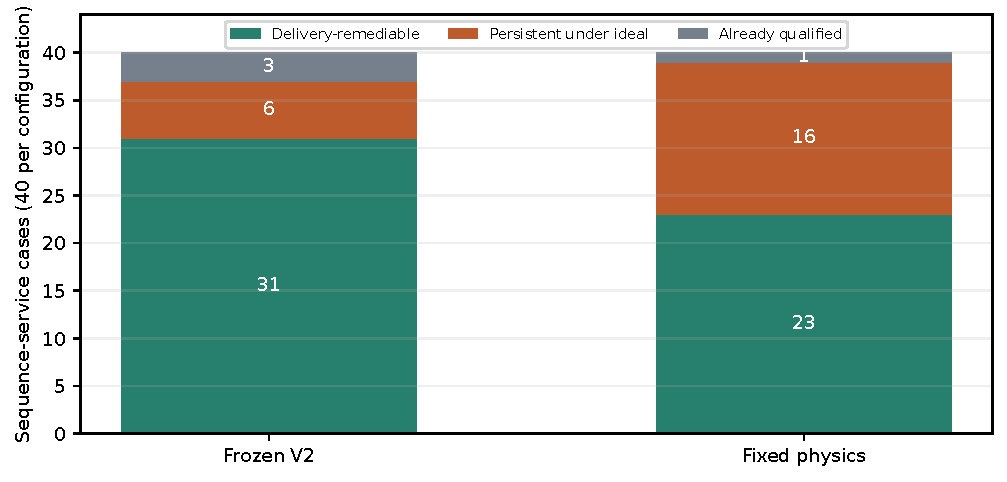
\includegraphics[width=.80\linewidth]{figures/frozen_configuration_remediability.pdf}
\caption{Remediability under frozen V2 and deterministic fixed physics.}
\end{figure}

\section{Lookahead, Deterministic Delivery, and Threshold Sensitivity}
\subsection{Centered-gradient lookahead as delay}
The centered-gradient implementation can require the next 10-Hz sensor sample. A predeclared 100-ms availability penalty was therefore added to every saved-state replay condition. The case partition changes from 30/6/4 to 31/6/3; only 1/40 sequence--service classifications changes. This is a latency sensitivity on existing trajectories, not a replacement for causal-feature retraining.

\subsection{Deterministic delay, jitter, and loss replay}
Deterministic replay over saved states realizes 10.001 Hz with zero loss for the ideal condition, 4.951 Hz with 0.987\% loss and mean p95 delay 82.8 ms for the practical condition, 1.900 Hz with 4.992\% loss and mean p95 delay 282.1 ms for the degraded condition, and 0.900 Hz with 9.991\% loss and mean p95 delay 463.6 ms for the stress condition. The emulated ledger is 32 remediable, six persistent, and two already qualified; the practical emulated condition restores 29 cases. This is deterministic delivery emulation, not measured network transport.

\subsection{Threshold curves}
One-factor-at-a-time sweeps use physical-tolerance multipliers 0.5--2.0, satisfaction requirements 0.60--0.95, and freshness-limit multipliers 0.5--1.5. The baseline ledger is reproduced at multiplier 1.0, while the partition changes under tighter and looser requirements. The ledger is therefore an operating-point result.

\begin{figure}[ht]\centering
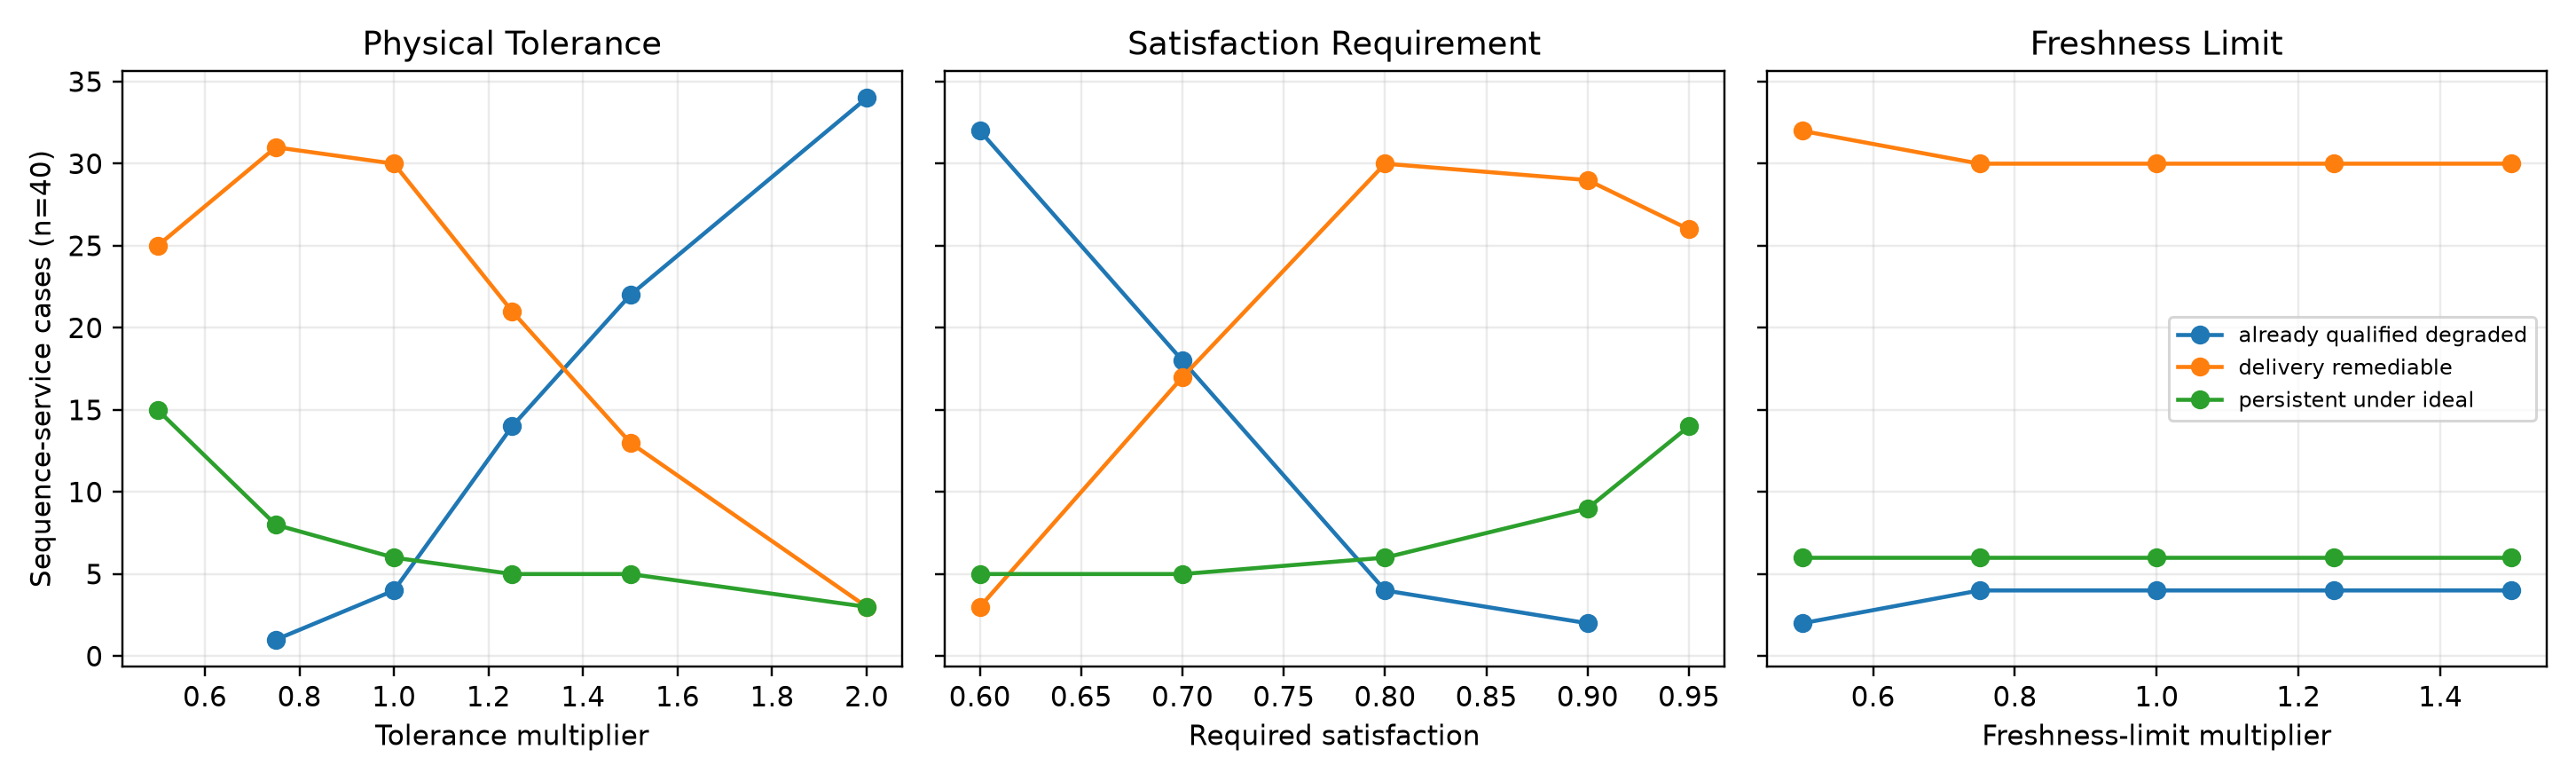
\includegraphics[width=.86\linewidth]{figures/threshold_curve_ledger.png}
\caption{Sequence-level remediability partition under physical-tolerance, satisfaction, and freshness-limit sweeps.}
\end{figure}

\begin{figure}[ht]\centering
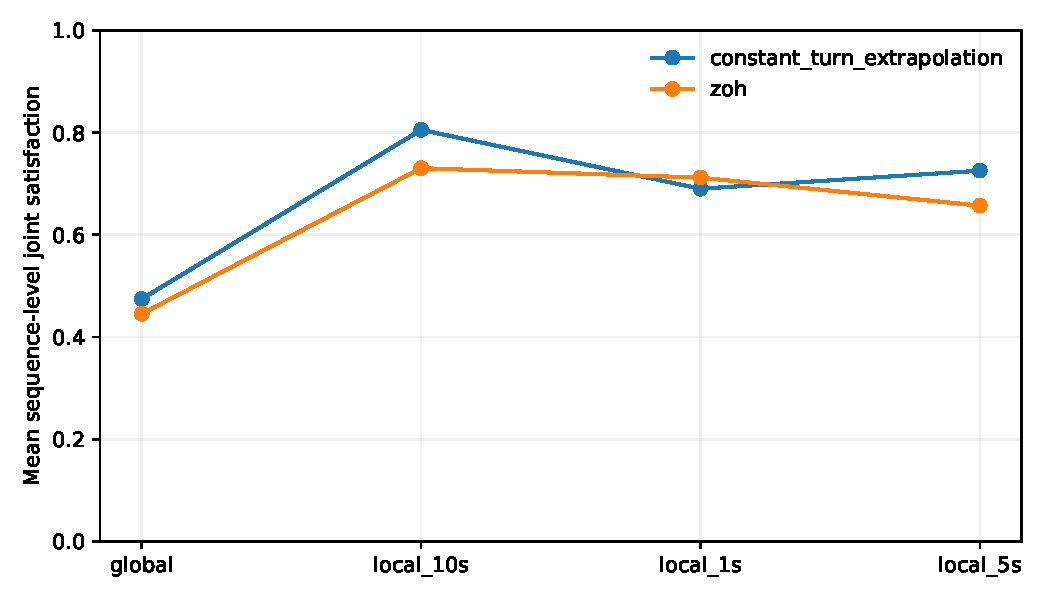
\includegraphics[width=.78\linewidth]{figures/receiver_robustness.pdf}
\caption{Zero-order hold and causal constant-turn receiver reconstruction sensitivity. Source phase remains nested within a physical sequence.}
\end{figure}

\section{UGV01 AprilTag Physical Instantiation}
The UGV01 physical-reference pipeline uses ChArUco camera calibration, fixed world tags, and a rover-mounted AprilTag. On the low-speed carpet development recording, asset-specific distance scale, asymmetric effective track widths, and bounded gyro contribution change ATE from 0.131 to 0.099 m, RPE$_1$ from 0.035 to 0.028 m, and heading MAE from $13.3^\circ$ to $5.6^\circ$. The repaired full-window fitted result is 0.114-m ATE, 0.030-m RPE$_1$, 0.087-m RPE$_5$, 0.104-m RPE$_{10}$, and $6.7^\circ$ heading MAE.

Frozen transfer to two August 29 holdouts is weak. Calibration-run ATE/heading MAE of 0.149 m/$21.2^\circ$ becomes 0.505 m/$76.3^\circ$ and 1.136 m/$108.7^\circ$. No tested common effective track width in 0.180--0.210 m reaches satisfaction 0.8 across all three runs.

Descriptive carpet, smooth-trapezoid, and smooth-square runs have ATE 0.114/0.101/0.338 m, heading MAE $6.7/17.4/28.6^\circ$, and corrected RPE$_1$ 0.029/0.023/0.017 m. The square contains a 20.935-s physical-reference gap; horizon pairs crossing it are excluded. Its corrected RPE$_5$/RPE$_{10}$ are 0.050/0.077 m while $D_p$ p95 is 0.918 m.

\begin{figure}[ht]\centering

\includegraphics[width=.84\linewidth]{figures/ugv01_rpe_vs_global_fidelity.png}
\caption{UGV01 finite-horizon RPE versus global ATE and $D_p$ p95 after reference-gap exclusion.}
\end{figure}

\begin{figure}[ht]\centering
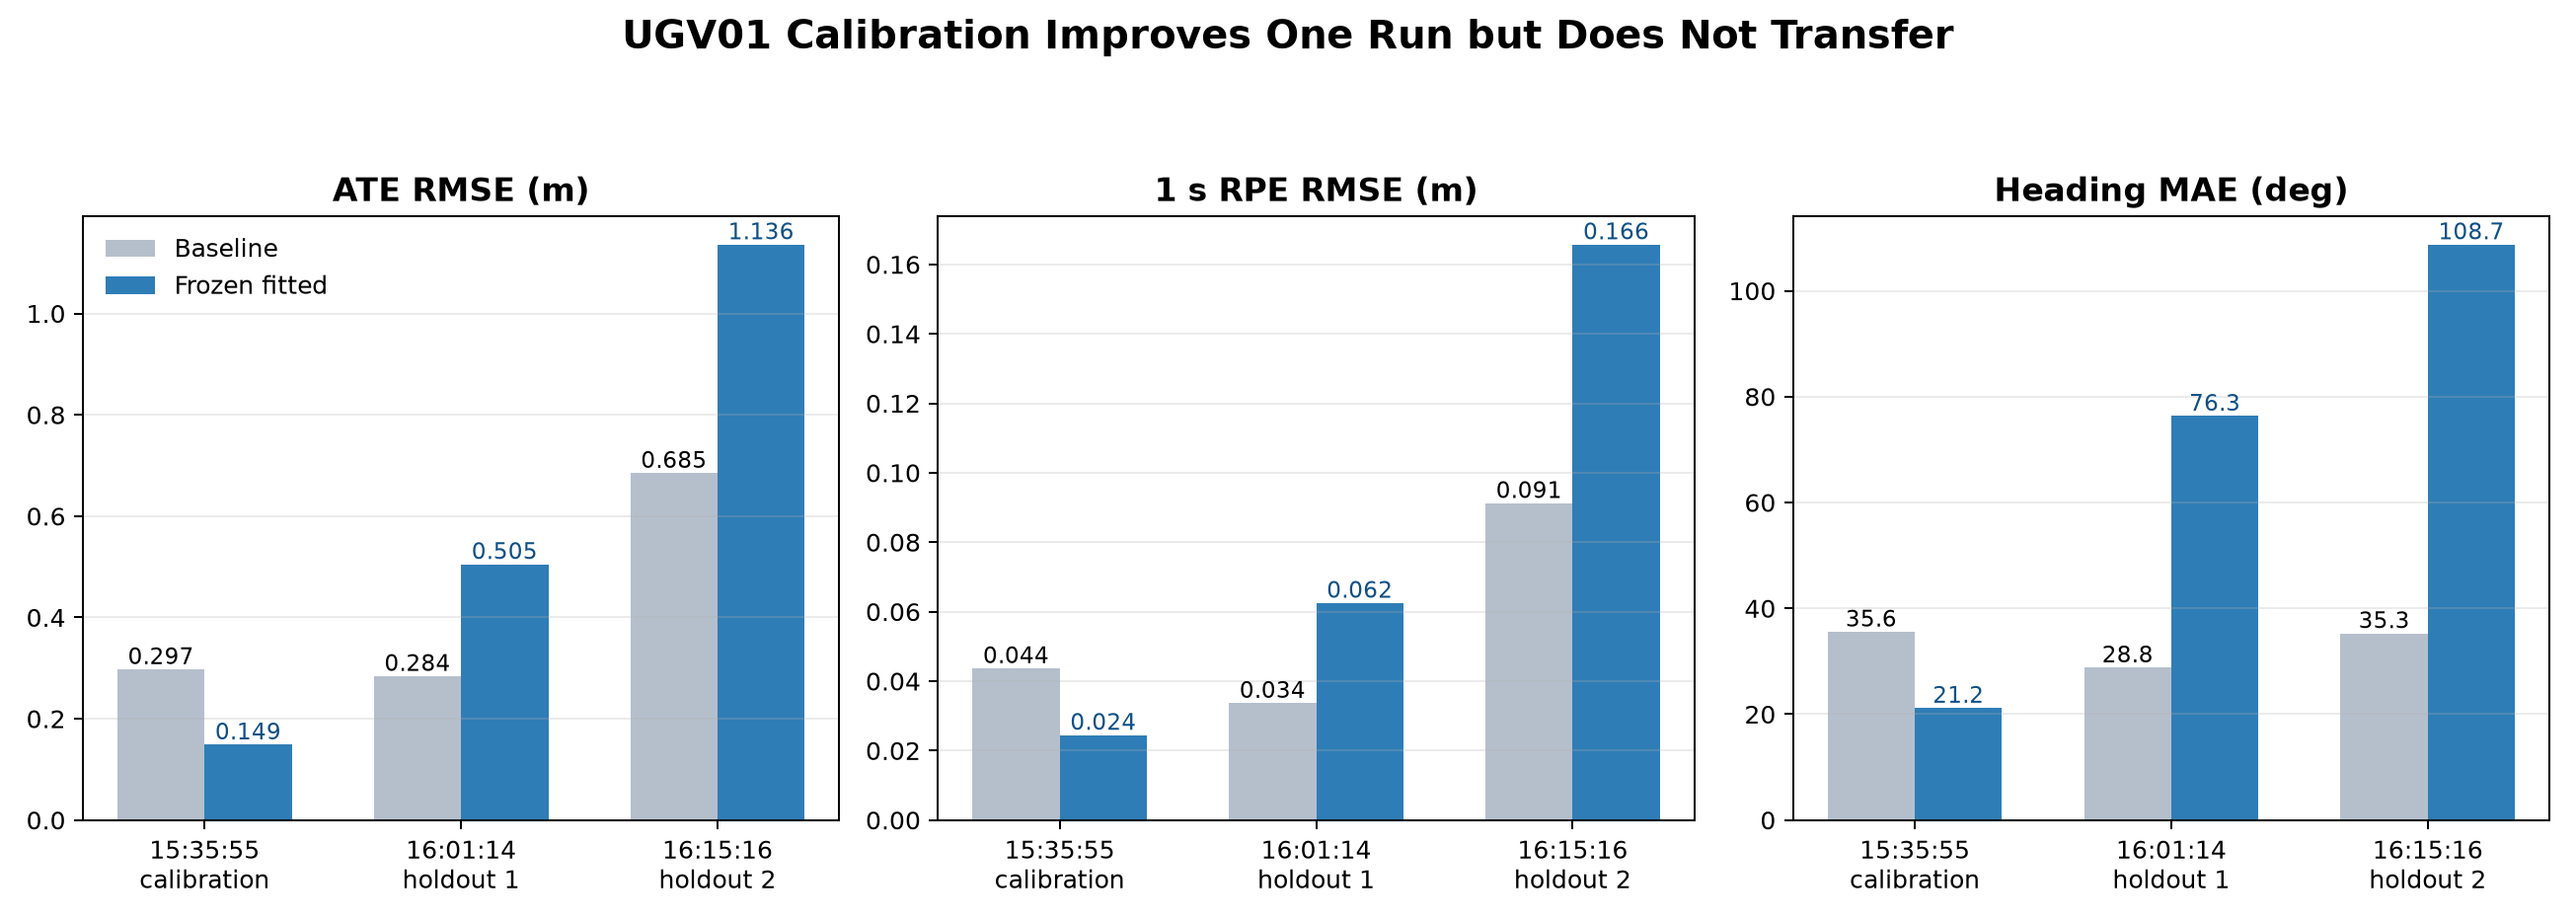
\includegraphics[width=.80\linewidth]{figures/ugv01_aug29_validation_summary.png}
\caption{UGV01 calibration recording and two frozen-parameter holdouts.}
\end{figure}

\section{TerraSentia External Platform}
Five TerraSentia sequences use valid RTK position as the primary positional reference. Dataset-provided fused EKF heading is used only for diagnostics. The deterministic adapter uses bag timestamps, local ENU conversion from the initial valid RTK origin, motor-side means, a nominal 0.26-m skid-steer yaw proxy, IMU yaw rate, and frozen i2Nav normalization.

Nominal-physics ATE spans 32.712--60.688 m and frozen-V2 median ATE spans 32.525--60.181 m. The corridor sequence is slightly worse under V2 (50.149 versus 49.904 m). Corrected physics RPE$_1$ spans 0.112--0.786 m. Oracle substitutions show that yaw accumulation is a major long-horizon contributor, but unresolved motor and IMU provenance prevents treating those substitutions as deployable models.

The unchanged position-service grid is nondegenerate on all five sequences. Frozen-V2 grid-average validity is 0.779, 0.421, 0.230, and 0.083 for local 1-s, local 5-s, local 10-s, and global position services. This demonstrates evaluator and contract portability; it does not demonstrate frozen-model portability.

\begin{figure}[ht]\centering

\includegraphics[width=.82\linewidth]{figures/E1_E2_cross_platform_position_contracts.png}
\caption{Position-contract feasibility across i2Nav and TerraSentia under the unchanged contract representation.}
\end{figure}

\section{UGV01 Live Telemetry and Trace Replay}
The live dataset contains 20/20 video, telemetry, and JSONL triplets across four requested-rate policies and five repetitions, totaling 2,702 JSONL records and 30.09 minutes on the rover source clock. Requested rates are 2 Hz for static-low, 10 Hz for static-high, mean 2.77 Hz for AoI-only, and mean 8.61 Hz for contract-aware. Delivered response rates cluster at 1.41--1.52 Hz because the serial HTTP path is the bottleneck.

The recorded dashboard used truncated elapsed time over long gaps, unrotated GPS/twin positions, stale qualification during outages, and a logged AoI relative to a minimum observed offset rather than verified absolute network age. Corrected code was tested later but was not deployed in these 20 runs. Low-speed GPS course also leaves position-plus-heading services frequently unobservable.

Trace-driven replay of five measured contract-aware service-time traces under four policy rules gives approximately 1.536 requests/s, 951.8 response bytes/s, and 1.304-s p95 delivery AoI for every policy. A fluid capacity study separates offered demand at a hypothetical 10 updates/s, but does not constitute measured communication or energy savings.

\begin{figure}[ht]\centering
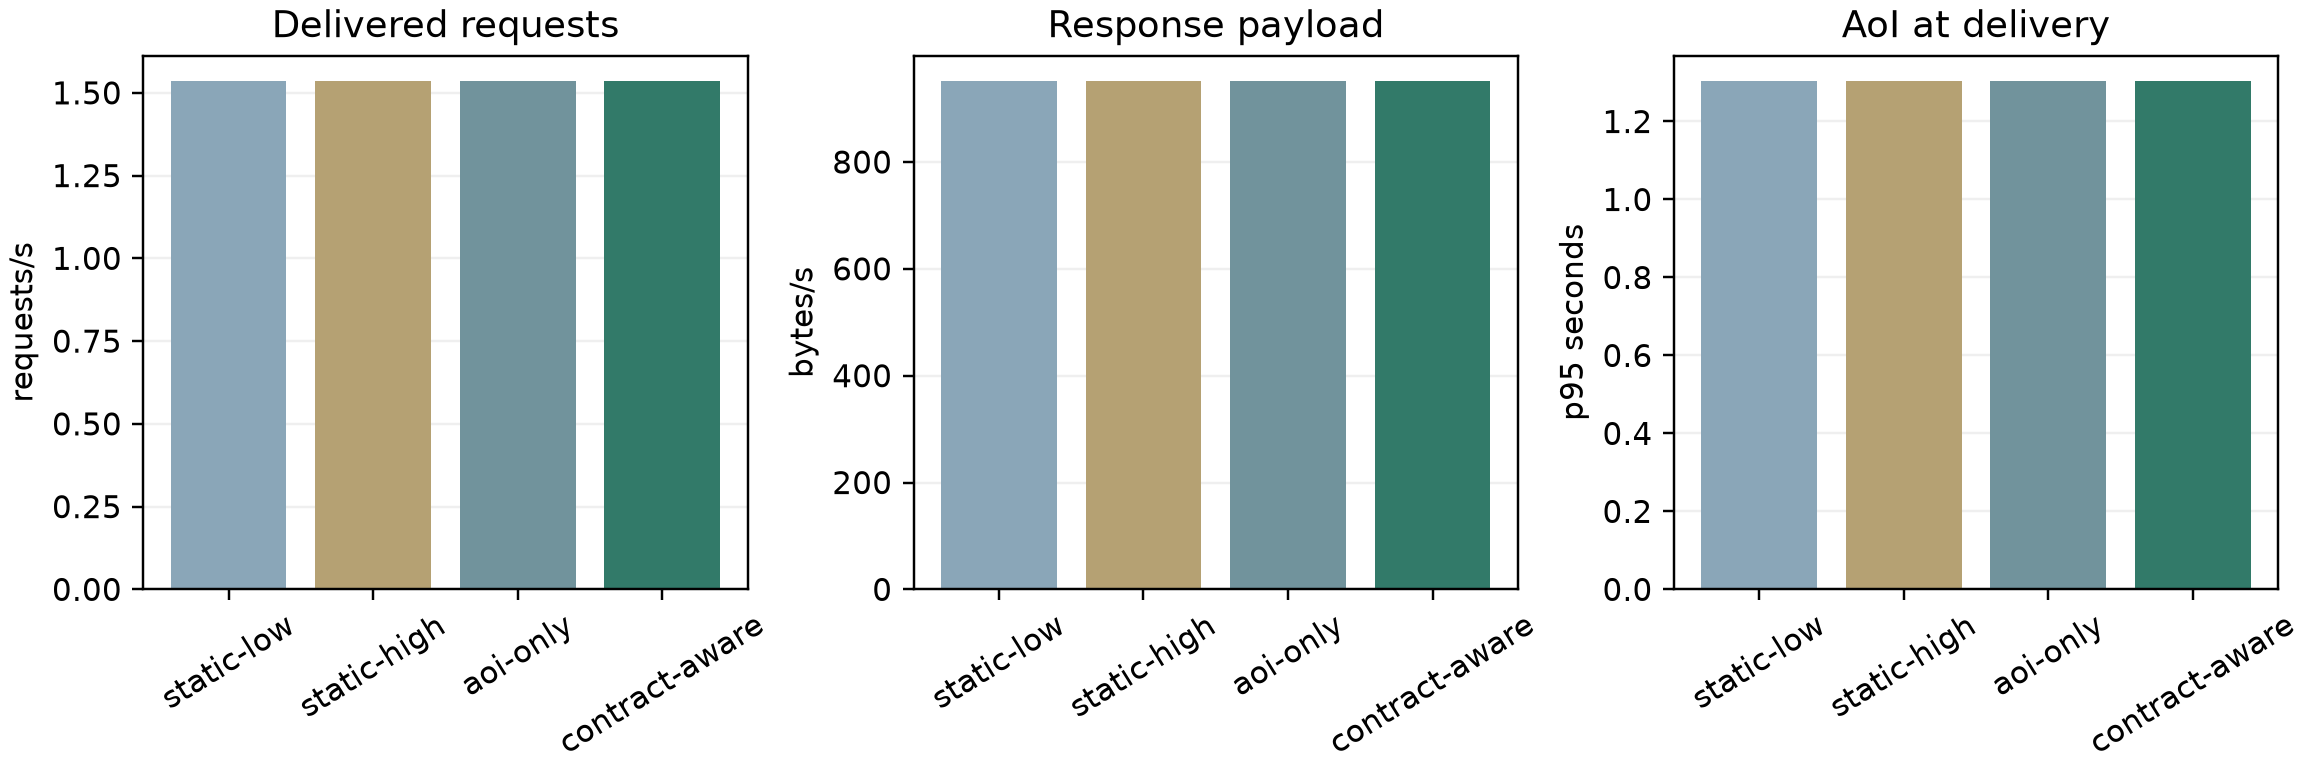
\includegraphics[width=.82\linewidth]{figures/trace_replay_policy_comparison.png}
\caption{Policy replay under the measured shared serial-HTTP service-time bottleneck.}
\end{figure}

\begin{figure}[ht]\centering
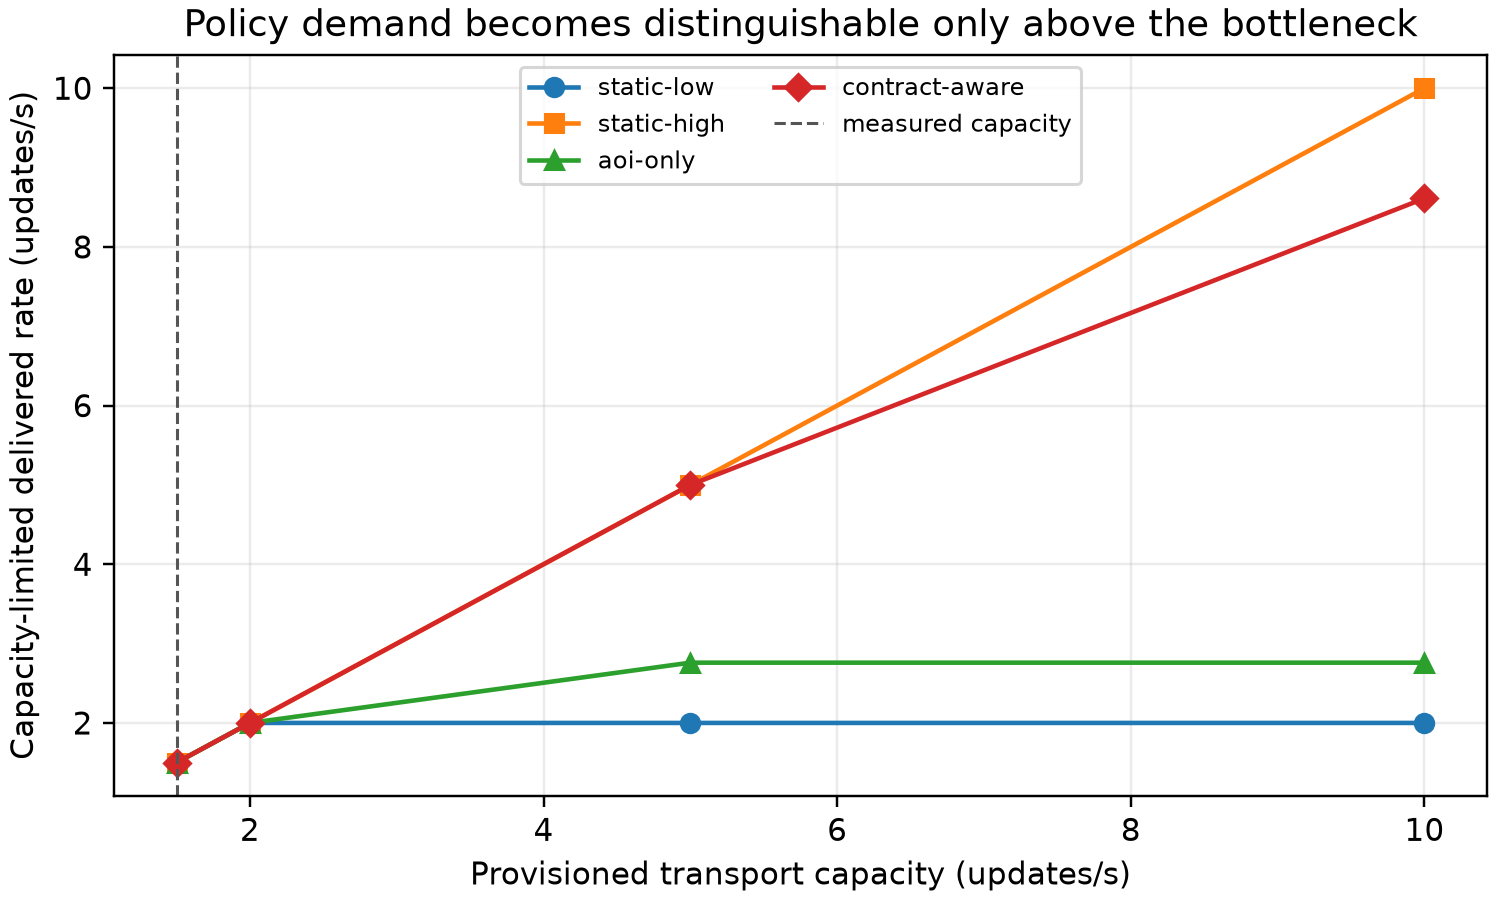
\includegraphics[width=.82\linewidth]{figures/transport_capacity_sensitivity.png}
\caption{Offered-demand sensitivity under hypothetical provisioned capacity.}
\end{figure}

\section{Cross-Domain Fidelity Experiments}
The component--horizon--tolerance contract is evaluated on MAGNET thermal forecasts, FreeTwinEV electro-thermal data, and TU Wien SNG process data using frozen 60/300/600-s target windows. Physical units and tolerances remain dataset-specific.

MAGNET contains 23 nonoverlapping paired windows. Median RMSE is $0.0876^\circ$C at within-window target-time offsets 0--60 s and $6.6176^\circ$C at offsets 301--599 s. The median paired increase is $6.0425^\circ$C with 95\% interval 2.2828--6.6952. The source records forecast target time but does not establish forecast issue or availability time, so no causal delivery, AoI, or remediability result is reported for MAGNET.

\begin{figure}[ht]\centering
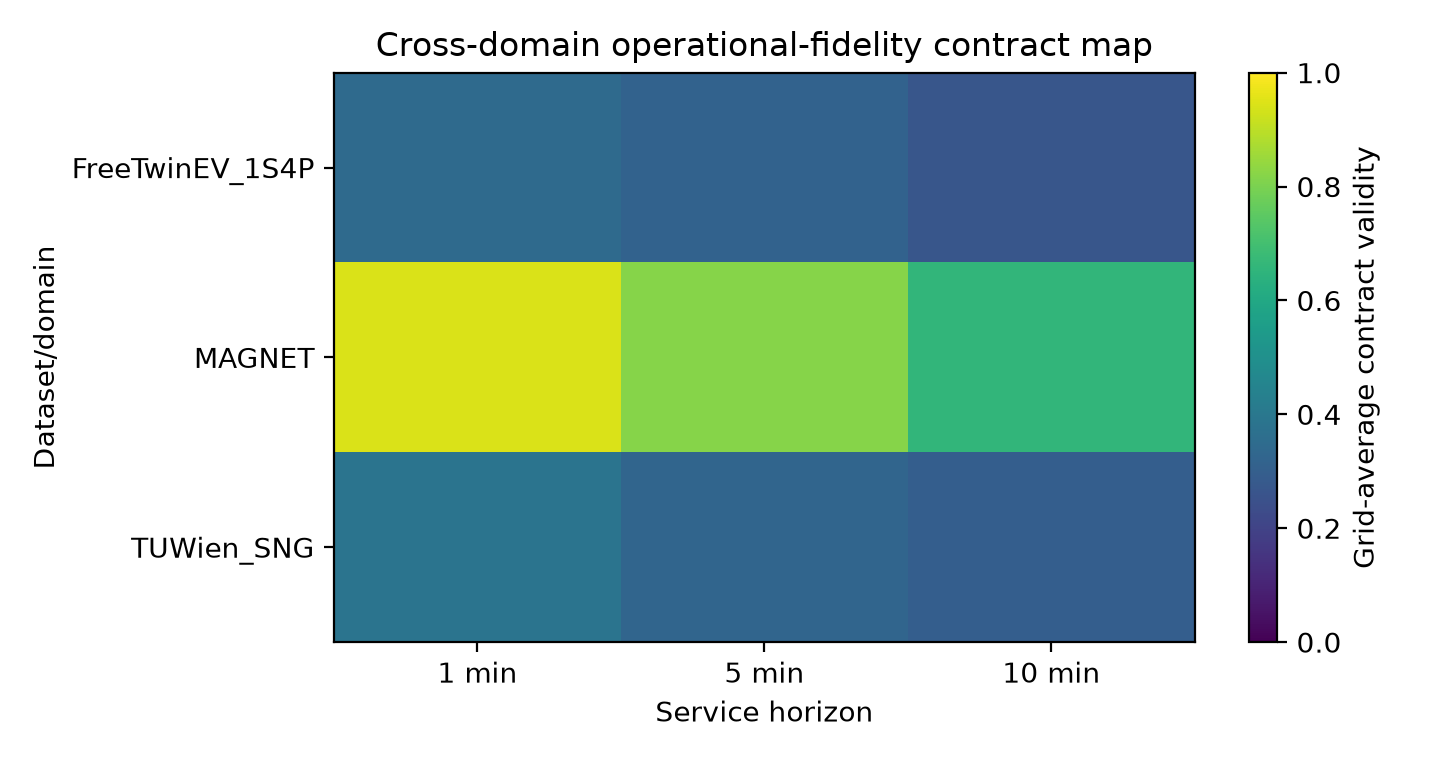
\includegraphics[width=.82\linewidth]{figures/cross_domain_contract_heatmap.png}
\caption{Cross-domain contract validity under normalized, dataset-specific tolerance grids.}
\end{figure}

\begin{figure}[ht]\centering
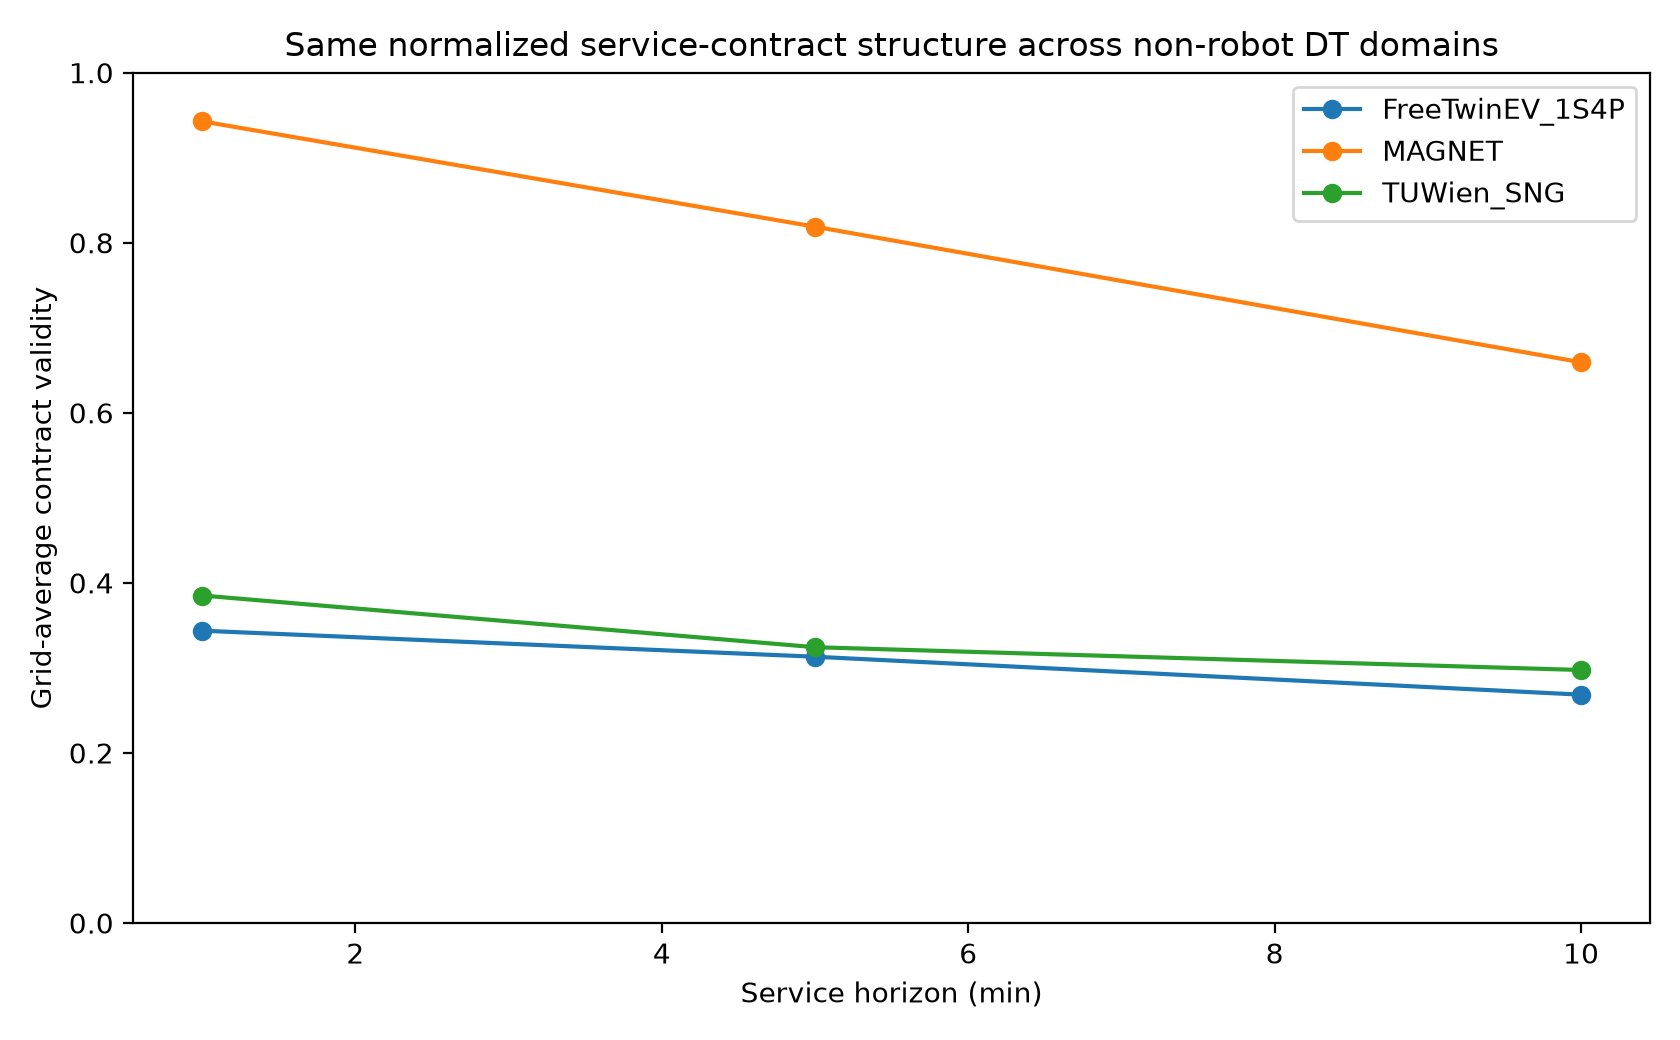
\includegraphics[width=.82\linewidth]{figures/cross_domain_horizon_profile.png}
\caption{Horizon-dependent fidelity across robot, thermal, battery, and process domains. MAGNET horizons are within-window target-time offsets.}
\end{figure}

\begin{figure}[ht]\centering
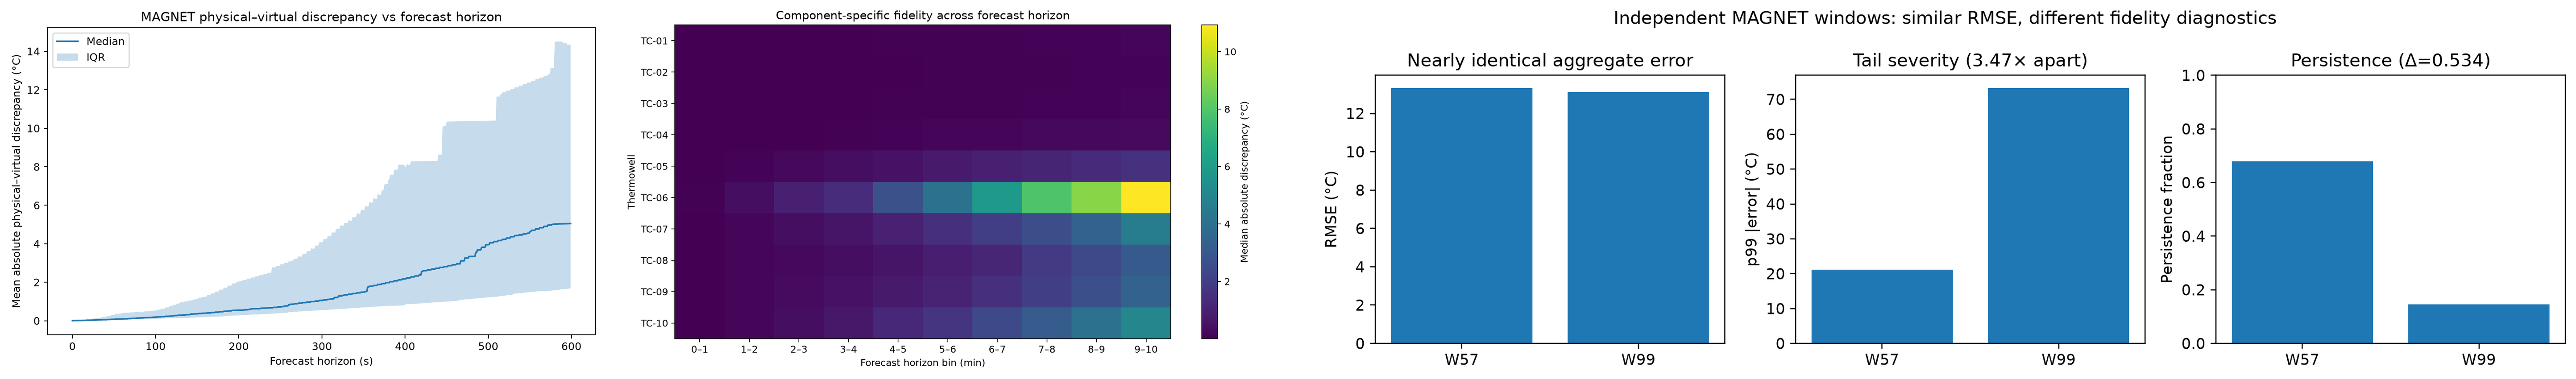
\includegraphics[width=.82\linewidth]{figures/magnet_horizon_component_counterexample.png}
\caption{MAGNET example in which aggregate error does not preserve component- and target-offset-specific behavior.}
\end{figure}

\section{Task-Level and Other Negative Experiments}
A causal position-only geofence replay uses a simulated 1-Hz independent physical reference delayed by 0.2 s. At the illustrative 1-m/1-s operating point, always-use releases nearly all answers with approximately 0.3\% error, while the full contract releases approximately 46\% with approximately 1.1\% error. Sparse occupancy and few boundary crossings prevent a task-protection conclusion.

Earlier delay and timestamp-jitter studies remain diagnostic. Delay changes state availability; timestamp jitter perturbs reported times. They are not equivalent interventions and do not establish live packet-level robustness.

\begin{figure}[ht]\centering
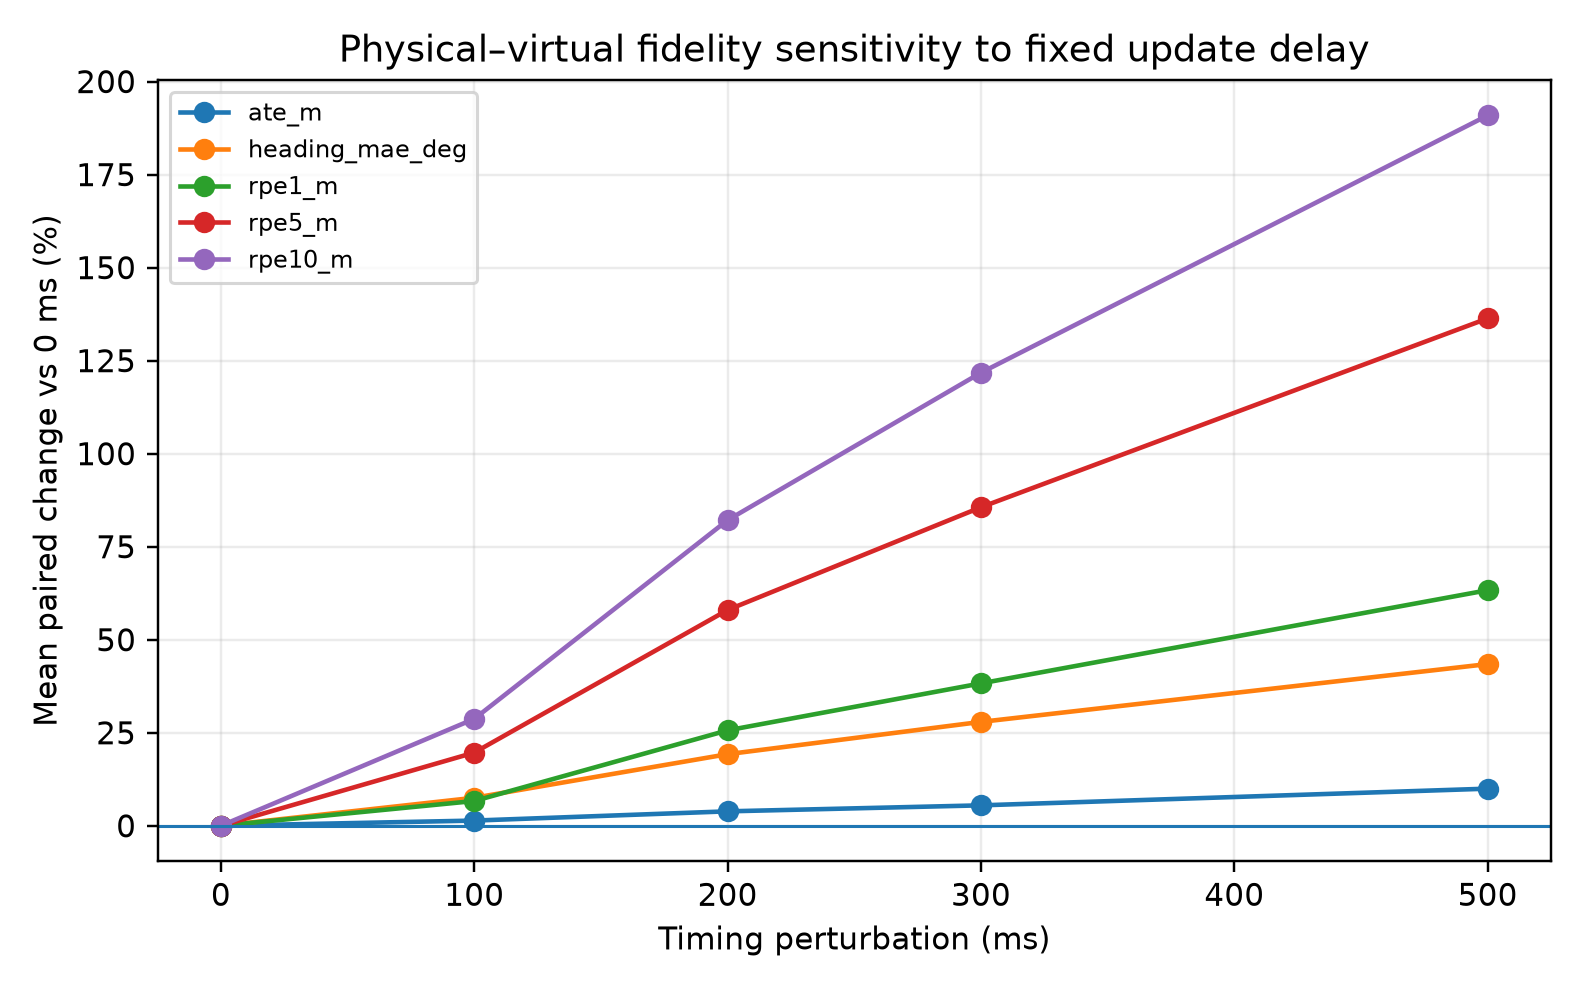
\includegraphics[width=.80\linewidth]{figures/timing_delay_stage2.png}
\caption{Saved-state delay sensitivity under its recorded replay protocol.}
\end{figure}

\begin{figure}[ht]\centering
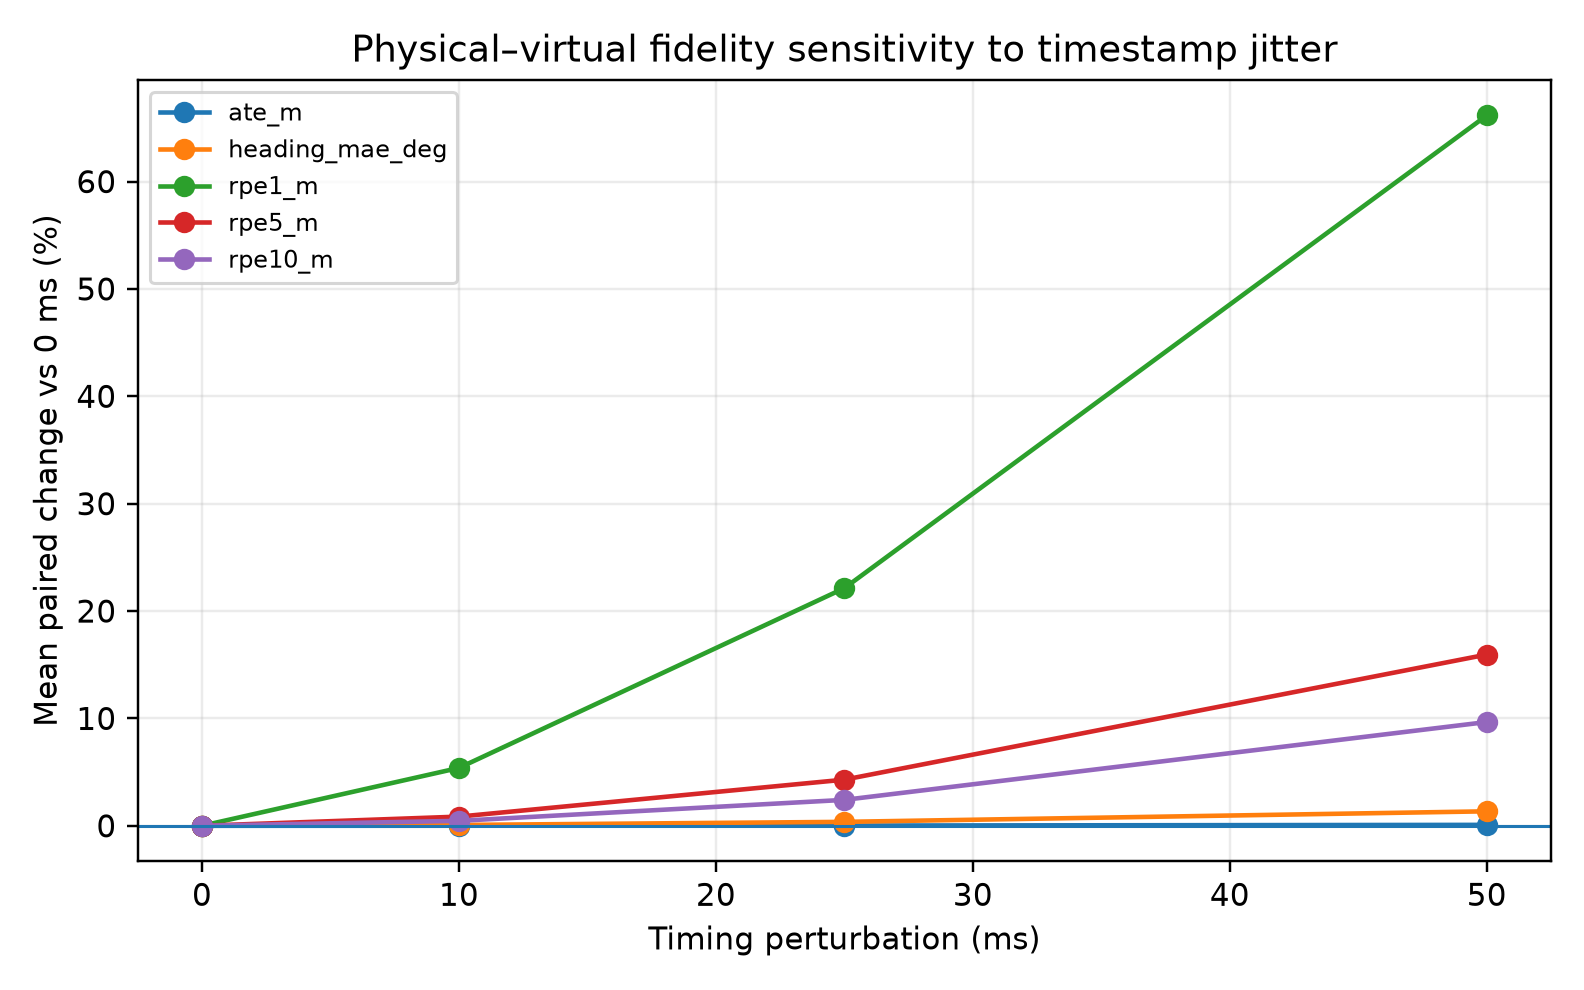
\includegraphics[width=.80\linewidth]{figures/timing_jitter_stage2.png}
\caption{Timestamp-jitter sensitivity, distinct from source-state arrival delay.}
\end{figure}

\section{Historical GPS-Security Replay}
The earlier security study uses 20 physical runs, three injection starts, and attack profiles to form 1,440 unique attack--run--start combinations. A later 14-detector table contains 20,160 detector--run evaluations; detector rows are not independent physical attacks. Paired replay shows that residual-coupled covariance adaptation can inflate process uncertainty, suppress normalized innovation scores, and increase undetected paired divergence. For standard drift against fixed covariance, the pooled NIS-ratio difference is $-0.251$, and maximum undetected paired error is 0.668 m larger. These are offline counterfactual replay results against a clean paired twin rather than live attacks or independent overhead ground truth.

\section{Legacy and Superseded Figures}
The following figures document earlier analysis stages. They are retained to preserve the experimental history but are not the numerical source for corrected timing counts. The five-column timing figure contains a 25/50-ms saved-clock alias, and the older matched-acceptance plot precedes the five-comparator correction.

\begin{figure}[ht]\centering
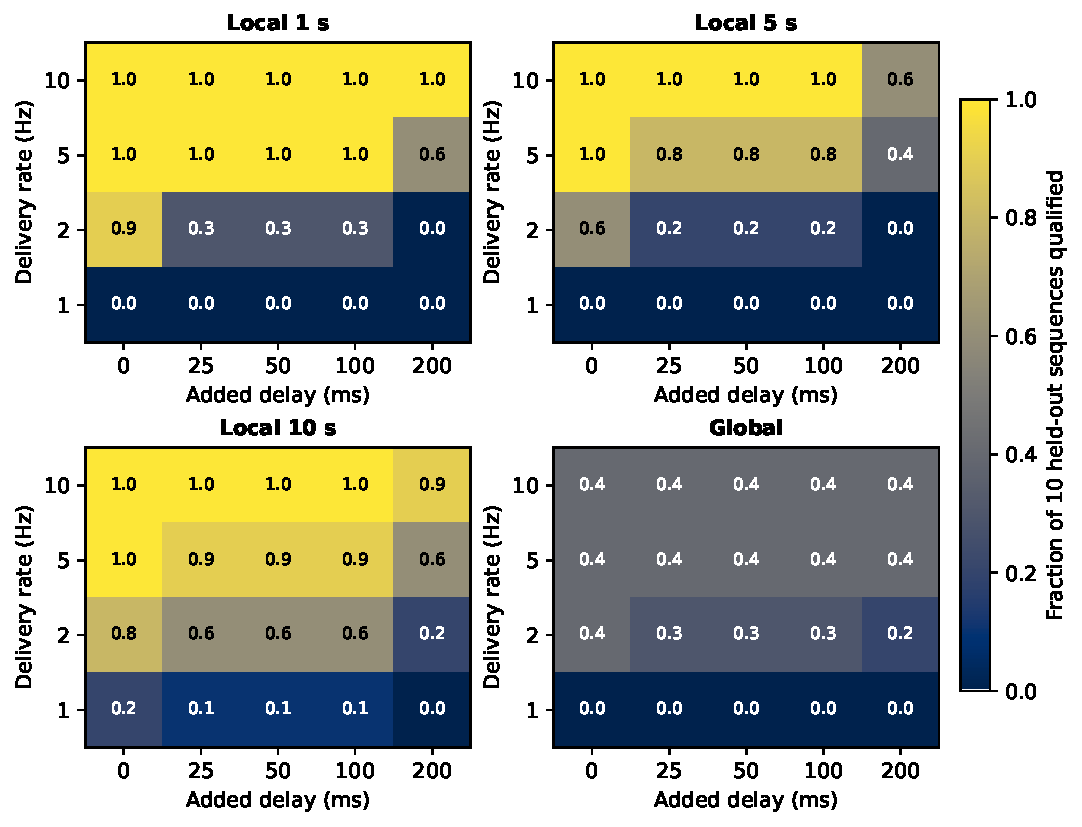
\includegraphics[width=.88\linewidth]{figures/timing_qualification_regions.pdf}
\caption{Legacy five-column timing surface. The 25- and 50-ms columns alias on the saved clock.}
\end{figure}

\begin{figure}[ht]\centering
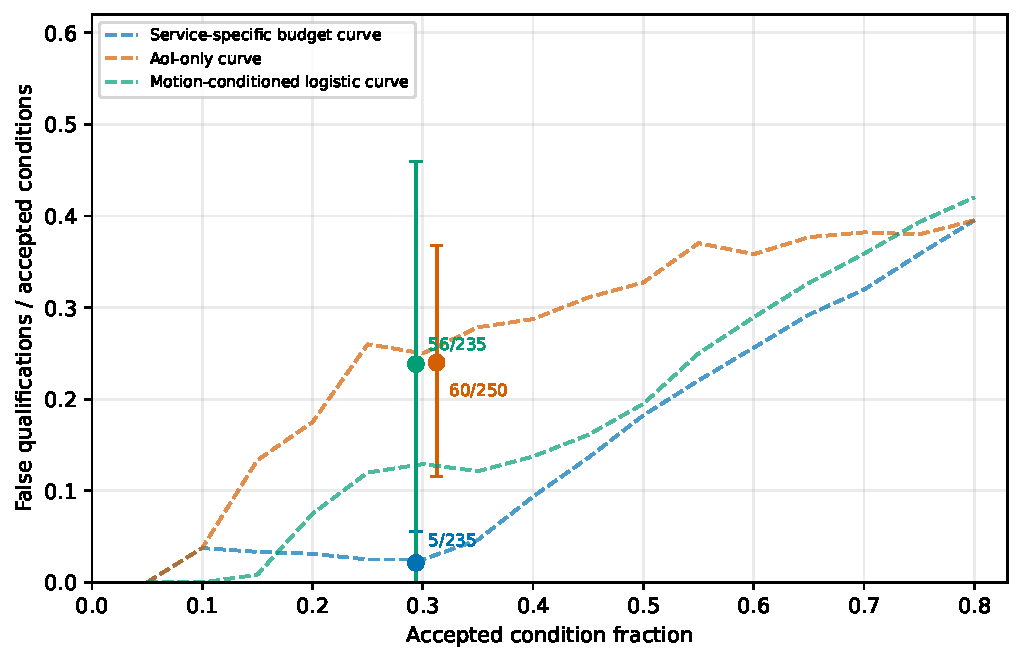
\includegraphics[width=.84\linewidth]{figures/matched_acceptance_false_qualification.pdf}
\caption{Legacy three-method matched-acceptance figure retained as an analysis-history artifact.}
\end{figure}

\section{Incomplete Experiments: Doubly Nested LOSO, Causal Features, and Linux Netem}
\label{app:pending}
\subsection{Doubly nested LOSO}
The corrected two-stage design defines an outer qualification-test sequence $u$. The checkpoint generating $u$ excludes $u$. Every qualification-training trajectory for another target sequence $v$ is generated by a checkpoint that excludes both $u$ and $v$ from training, normalization fitting, validation, and checkpoint selection as applicable. The complete design has 10 outer sequences, 3 seeds, and 10 trajectories per outer fold, totaling 300 V1-to-V2 pipelines.

The supplied archive \path{i2nav_doubly_nested_full10_shard_00_of_60.zip} is one of 60 shards. Its audit passes five tasks at repository commit \texttt{6f91f5d}, all for seed 42. It includes outer-test trajectories for building00, building02, parking01, playground00, and street01 with recorded split provenance and SHA-256 hashes. This shard is complete, but the full experiment is not: 59 shards and the aggregate trajectory-bank audit remain outstanding. No corrected qualification surface, comparator result, or remediability ledger is inferred from this partial shard.

\subsection{Causal-derivative LOSO}
The causal-feature experiment replaces centered derivatives with backward derivatives and includes a numerical no-lookahead preflight. It contains 30 ordinary LOSO tasks and tests whether causal feature construction changes the frozen-model conclusions. It does not repair the two-stage qualification split by itself.

The supplied archive \path{i2nav_v2_causal_derivative_shard_00_of_06.zip} is one of six shards. Its audit passes five seed-42 tasks for building00, building02, parking01, playground00, and street01 at commit \texttt{6f91f5d}. Five shards and aggregate analysis remain outstanding. The existing 100-ms lookahead-as-delay sensitivity remains the only completed lookahead result until the full causal bank is merged.

\subsection{Linux netem}
The Linux experiment sends identifiers for precomputed frozen states through an isolated virtual Ethernet pair and network namespace shaped by \texttt{tc netem}. It records monotonic send and arrival times, packet loss, realized delay, and requested versus realized rate. The planned full run uses four delivery conditions, three 180-s transport repetitions, and applies each measured trace to the existing physical-sequence trajectories. Transport repetitions quantify network variability and do not increase the number of physical sequences.

This experiment has not been run. Its intended result is OS-level emulated delivery over precomputed states. It will not be described as live inference, measured energy savings, or a safety experiment. The current deterministic delay/jitter/loss replay in the preceding appendix is a separate completed software emulation.

\section{Artifact Registry}
\begin{longtable}{p{.37\linewidth}p{.18\linewidth}p{.35\linewidth}}
\caption{Major experiment families and evidence types. Paths are relative to \texttt{results/}.}\label{tab:registry}\\
\toprule
Artifact root & Evidence type & Contents \\
\midrule\endfirsthead
\toprule
Artifact root & Evidence type & Contents \\
\midrule\endhead
\path{i2nav_v2_full_loso} & Frozen model & Thirty V2 runs, ten sequences, three seeds. \\
\path{i2nav_frozen_v2_fidelity_analysis} & Fidelity analysis & Mechanism, conditions, profiles, and envelopes. \\
\path{benign_envelope_validation} & Held-out analysis & Conditioned/unconditional coverage and stability. \\
\path{i2nav_official_benchmark} & Benchmark & Official-format APE/RPE evaluation. \\
\path{service_timing_budget} & Saved-state replay & Service surfaces and historical case ledger. \\
\path{service_timing_reviewer_checks} & Comparator audit & Acceptance, selective risk, and case accounting. \\
\path{service_timing_robustness} & Sensitivity & Receiver, phase, and fixed-physics comparisons. \\
\path{lookahead_as_delay_sensitivity} & Sensitivity & 100-ms feature-availability penalty. \\
\path{deterministic_delivery_replay} & Software emulation & Delay, jitter, loss, realized rates, and ledger. \\
\path{service_threshold_curve_ledger} & Sensitivity & Tolerance, satisfaction, and freshness curves. \\
\path{e1_e2_service_contract_publication} & Cross-platform & Metric rank inversions and TerraSentia contracts. \\
\path{e1_rank_inference} & Statistical audit & Dependence-aware local/global rank analysis. \\
\path{service_relative_fidelity} & Negative study & Condition-aware monitor versus unconditional support. \\
\path{service_risk_estimator_nested_loso} & Negative study & Causal service-risk estimator and no-go checks. \\
\path{ugv01_physical_instantiation} & Physical reference & AprilTag calibration, conditions, and holdouts. \\
\path{ugv01_contract_parameter_study} & Parameter study & Track-width interval and cross-run contract sensitivity. \\
\path{ugv01_live_position_contract} & Observability sensitivity & Position-only GPS contract replay. \\
\path{ugv01_live_contract_experiment} & Prototype & Initial single-run live dashboard experiment. \\
\path{ugv01_live_contract_dataset_audit} & Live traces & Twenty-run telemetry/video/JSONL audit. \\
\path{ugv01_live_contract_trace_replay} & Trace replay & Serial transport and capacity sensitivity. \\
\path{terrasentia_external_validation} & External platform & Five RTK-referenced sequences and 30 checkpoints. \\
\path{aifarms_terrasentia_phase2} & Adapter audit & Timestamp, feature, frame, and oracle diagnostics. \\
\path{terrasentia_timing_diagnostic} & Timing diagnostic & External-platform saved-state timing checks. \\
\path{cross_domain_contract_generalization} & Cross-domain & MAGNET, FreeTwinEV, and TU Wien SNG. \\
\path{magnet_tfp} & Thermal fidelity & Target-offset component and persistence analysis. \\
\path{magnet_timing_provenance} & Provenance stop & No verified issue/availability time. \\
\path{geofence_decision_value} & Negative task study & Position-only decision replay. \\
\path{i2nav_fidelity_metric_comparison} & Evaluator comparison & ATE/RPE, path geometry, traces, and fidelity profiles. \\
\path{munoz_trace_alignment} and \path{tfp_vs_munoz} & Method comparison & Trace alignment versus synchronized component fidelity. \\
\path{sensing_fidelity_comparison} & Sensor comparison & Sensing burden and protocol-compatible accuracy. \\
\path{iot_resource_characterization} & Resource audit & Parameter count and serialized checkpoint footprint. \\
\path{i2nav_adaptive_q} and \path{i2nav_gru_dualhead} & Model development & Learned uncertainty and residual-model experiments. \\
\path{i2nav_parking00}, \path{i2nav_playground00}, and \path{i2nav_street00} & Model development & Per-sequence MLP/tree/boosting bakeoffs. \\
\path{i2nav_baseline_methods} and \path{i2nav_final_model_study*} & Model development & Baselines, physics revisions, and pre-freeze studies. \\
\path{i2nav_loso_ablation} and \path{i2nav_context_length_identifiability} & Ablation & Architecture and context-length experiments. \\
\path{i2nav_physics_residual_diagnostics} and \path{i2nav_timing_sensitivity} & Diagnostics & Residual mechanism and timing analyses. \\
\path{i2nav_v1_frozen} and \path{i2nav_v1_legacy_10fold_3seed} & Historical model & V1 fold and provenance artifacts. \\
\path{i2nav_v2_bias_diagnostic} and V2 pilot roots & Pilot models & Yaw-bias, fast-neutral, and slow-additive tests. \\
\path{i2nav_predictive_nll_pilot_v3*} & Pilot models & Predictive-NLL training sensitivities. \\
\path{i2nav_zero_shot_observable_audit*} & Adapter audits & Observable-feature, sign, and yaw variants. \\
\path{covariance_poisoning} and \path{expanded_grid} & Security replay & Historical GPS manipulation studies. \\
\path{replicate_01_base42}, \path{replicate_02_base1042}, and \path{replicate_03_base2042} & Historical output & Earlier per-seed generated results. \\
\path{publication_hardening}, \path{result_freeze_audit}, and \path{results_quality_review} & Evidence audit & Numerical, provenance, and claim consistency checks. \\
\path{frozen_result_manifest} and \path{manuscript_results_dossier} & Packaging & Result registry and document-support artifacts. \\
\path{doubly_nested_loso} & Incomplete & Partial imported-bank placeholder; no aggregate result. \\
\path{causal_derivative_loso} & Incomplete & Partial imported-bank placeholder; no aggregate result. \\
\bottomrule
\end{longtable}

\section*{Conclusion}
The experiments establish that digital-twin fidelity is multidimensional, horizon-dependent, condition-dependent, and service-relative. Short-horizon trajectory agreement does not guarantee global synchronization. In the i2Nav study, persistent yaw mismatch is strongly associated with accumulated yaw residual, and heading divergence is strongly associated with position divergence. Condition variables change both local and global fidelity distributions, while difficult parking sequences dominate global position and heading tails.

Service contracts provide a common representation for physical discrepancy, freshness, and observability. Saved-state replay shows how a newer delivered state can restore qualification without changing the model, while persistent cases remain unqualified under ideal delivery. The historical timing and comparator counts remain qualification-label-held-out results until the complete doubly nested trajectory bank is available. The 100-ms lookahead sensitivity, deterministic delay/jitter/loss replay, and threshold curves quantify how the ledger changes under explicit timing and requirement perturbations.

The physical and external experiments define the boundaries of the result. UGV01 AprilTag data support accurate same-run asset-specific calibration but show poor transfer to two frozen holdouts. TerraSentia supports evaluator and contract portability while showing weak frozen-model portability and unresolved sensor provenance. The live UGV01 traces demonstrate a transport bottleneck that collapses requested policy rates. MAGNET, FreeTwinEV, and TU Wien SNG support structural contract portability, while MAGNET lacks the timing provenance required for causal delivery analysis.

The remaining computational work is explicit: merge all 60 doubly nested shards, merge all six causal-derivative shards, rerun service evidence only after both banks pass provenance audits, and execute the Linux \texttt{netem} transport study. Until those experiments finish, partial archives are provenance evidence rather than aggregate experimental results.

\begin{thebibliography}{99}
\bibitem{jones2020} D. Jones \emph{et al.}, Characterising the Digital Twin: A systematic literature review, \emph{CIRP Journal of Manufacturing Science and Technology}, vol. 29, pp. 36--52, 2020, doi: 10.1016/j.cirpj.2020.02.002.
\bibitem{shao2023} G. Shao, J. Hightower, and W. Schindel, Credibility consideration for digital twins in manufacturing, \emph{Manufacturing Letters}, vol. 35, pp. 24--28, 2023, doi: 10.1016/j.mfglet.2022.11.009.
\bibitem{munoz2024} P. Mu\~noz \emph{et al.}, Measuring the Fidelity of a Physical and a Digital Twin Using Trace Alignments, \emph{IEEE Transactions on Software Engineering}, vol. 50, no. 12, pp. 3122--3145, 2024, doi: 10.1109/TSE.2024.3462978.
\bibitem{bergs2025} L. Bergs \emph{et al.}, Evaluating mobile robot navigation behavior in flexible assembly systems through digital twin and real-world experiments, \emph{Discover Robotics}, vol. 1, Art. no. 10, 2025, doi: 10.1007/s44430-025-00010-4.
\bibitem{maatouk2023} A. Maatouk, M. Assaad, and A. Ephremides, The Age of Incorrect Information: An Enabler of Semantics-Empowered Communication, \emph{IEEE Transactions on Wireless Communications}, vol. 22, no. 4, pp. 2621--2635, 2023, doi: 10.1109/TWC.2022.3213227.
\bibitem{chiariotti2022} F. Chiariotti \emph{et al.}, Query Age of Information: Freshness in Pull-Based Communication, \emph{IEEE Transactions on Communications}, vol. 70, no. 3, pp. 1606--1622, 2022, doi: 10.1109/TCOMM.2022.3141786.
\bibitem{tanmatta2024} B. Tan and A. Matta, The digital twin synchronization problem: Framework, formulations, and analysis, \emph{IISE Transactions}, vol. 56, no. 6, pp. 652--665, 2024, doi: 10.1080/24725854.2023.2253869.
\bibitem{li2025sync} Y. Li \emph{et al.}, Budget-Constrained Digital Twin Synchronization and Its Application on Fidelity-Aware Queries in Edge Computing, \emph{IEEE Transactions on Mobile Computing}, vol. 24, no. 1, pp. 165--182, 2025, doi: 10.1109/TMC.2024.3455357.
\bibitem{brossard2019} M. Brossard and S. Bonnabel, Learning Wheel Odometry and IMU Errors for Localization, in \emph{Proc. IEEE ICRA}, 2019, pp. 291--297, doi: 10.1109/ICRA.2019.8794237.
\bibitem{jiang2025} C. Jiang \emph{et al.}, WING: Wheel-Inertial Neural Odometry with Ground Manifold Constraints, \emph{IEEE Transactions on Intelligent Vehicles}, vol. 10, no. 3, pp. 1510--1525, 2025, doi: 10.1109/TIV.2024.3429167.
\bibitem{zhou2025ynet} P. Zhou \emph{et al.}, Learning Yaw Velocity for Inertial-Wheel Odometry on Autonomous Vehicles, \emph{IEEE Transactions on Intelligent Vehicles}, vol. 10, no. 5, pp. 3517--3530, 2025, doi: 10.1109/TIV.2024.3455566.
\bibitem{tang2025} H. Tang \emph{et al.}, i2Nav-Robot: A Large-Scale Indoor-Outdoor Robot Dataset for Multi-Sensor Fusion Navigation and Mapping, arXiv:2508.11485, 2025, doi: 10.48550/arXiv.2508.11485.
\bibitem{cuaran2024} J. Cuaran \emph{et al.}, Under-canopy dataset for advancing simultaneous localization and mapping in agricultural robotics, \emph{The International Journal of Robotics Research}, vol. 43, no. 6, pp. 739--749, 2024, doi: 10.1177/02783649231215372.
\bibitem{olson2011} E. Olson, AprilTag: A robust and flexible visual fiducial system, in \emph{Proc. IEEE ICRA}, 2011, pp. 3400--3407, doi: 10.1109/ICRA.2011.5979561.
\bibitem{wilsdon2023magnet} K. Wilsdon \emph{et al.}, Autonomous control of heat pipes through digital twins: Application to fission batteries, \emph{Progress in Nuclear Energy}, vol. 163, Art. no. 104813, 2023, doi: 10.1016/j.pnucene.2023.104813.
\end{thebibliography}
\end{document}
